% !TeX program = PdfLaTeX
% !TeX encoding = ISO-8859-1
% !TeX spellcheck = es_ES, en_US




\documentclass[a4paper,12pt]{book}
  
	\usepackage{ae}
	\usepackage[T1]{fontenc}
	\usepackage{geometry}
	\usepackage{graphicx} 
	\usepackage{wrapfig}
	\graphicspath{ {figuras/} } 
	\usepackage{fancyhdr} 
	\usepackage{sectsty}
	\usepackage{tocloft}
	\usepackage[nopostdot,style=super,nonumberlist,toc]{glossaries}
	\usepackage{float}
	\restylefloat{table}
	\usepackage{titlesec}
	\usepackage[spanish]{babel}
	\usepackage{apacite}
	\usepackage{url}
	\usepackage{enumitem}


\titleformat{\chapter}[display]
{\normalfont\bfseries}{}{0pt}{\Large}

	%Centra el titulo de los capitulos
	\chapterfont{\centering}
	%Centra el titulo de las secciones
	%\sectionfont{\centering}
	%Centra el titulo de las sub-secciones
	%\subsectionfont{\centering}
	
	

	
	%Usar cuando queremos ver el area de impresion(muy bueno)
	%\usepackage{showframe}
	
	
	%Configura el footer con numeros de pagina CE=CENTER EVENT, CO=CENTER ODD
	%%\pagestyle{fancy}	
	%%\fancyhf{}
	%%\fancyfoot[CE,CO]{\ifnum\value{page}<17\relax\else\thepage\fi}
	%elimina el subrayado del header
	%%\renewcommand{\headrulewidth}{0pt}
	%muestra un subrayado despues del footer
	%\renewcommand{\footrulewidth}{0.4pt}
	
	
	% Page style for preliminary pages.
	\fancypagestyle{preliminary}{
		\fancyhf{}% Clear header/footer
		\fancyfoot[C]{\thepage}% Footer
		\renewcommand{\headrulewidth}{0pt}% No header rule
	}
	
	% Page style for main matter.
	\fancypagestyle{mainmatter}{
		\fancyhf{}% Clear header/footer
		\fancyfoot[C]{\thepage}% Footer
		\renewcommand{\headrulewidth}{0pt}% No header rule
	}
	
	
	% Glosario
	%\usepackage[doublespacing]{setspace}
	
	\setlength{\glsdescwidth}{0.9\linewidth}
	\newglossarystyle{mylong}{
		\glossarystyle{long}
		\renewcommand*{\glossaryentryfield}[5]{%
			\glsentryitem{##1}\glstarget{##1}{##2} & ........................ ##3\glspostdescription\space ##5\\[8pt]}%
		\renewcommand{\glsgroupskip}{}
	}
	\makeglossaries% Inicia

	
	\begin{document}
		\pagestyle{preliminary}\pagenumbering{roman}
		\fancypagestyle{plain}{\pagestyle{preliminary}}% Correct plain page style
		
		%Cubiertas o tapas del libro
		
\begin{center}
	
\includegraphics[width=30mm]{figuras/uca.png}
\end{center}	

\begin{center}
	\fontsize{16}{16}\selectfont
	UNIVERSIDAD CATOLICA\\
	``NUESTRA SE�ORA DE LA ASUNCI�N"\\
	CAMPUS ALTO PARAN�\\
	\fontsize{14}{14}\selectfont
	FACULTAD DE CIENCIAS Y TECNOLOG�A
\end{center}


\vspace*{2\baselineskip}
\begin{center}
	\textbf{DATA DISCOVERY APLICADOS A DATOS DEL PARAGUAY}
\end{center}

\vspace*{2\baselineskip}
\begin{center}
	\fontsize{12}{12}\selectfont
	Proyecto Final de Graduaci�n presentado a la Facultad de Ciencias y
	Tecnolog�a como requisito obligatorio para la obtenci�n del t�tulo de
	Lic. en An�lisis de Sistemas
\end{center}

%3 saltos de linea
\vspace*{3\baselineskip}
\begin{center}
	\textbf{Ariel Hern�n Landaida Duarte\\
	Iv�n Ariel C�ceres Ca�ete}
\end{center}


%llena el espacio vacio
\vfill
\begin{center}
	Hernandar�as, diciembre de 2015
\end{center}



		\clearpage\null
		\begin{center}
	\fontsize{16}{16}\selectfont
	UNIVERSIDAD CATOLICA\\
	``NUESTRA SE�ORA DE LA ASUNCI�N"\\
	CAMPUS ALTO PARAN�\\
	\fontsize{14}{14}\selectfont
	FACULTAD DE CIENCIAS Y TECNOLOG�A
\end{center}
\vspace*{5\baselineskip}
\begin{center}
	\textbf{DATA DISCOVERY APLICADOS A DATOS DEL PARAGUAY}
\end{center}
\vspace*{5\baselineskip}
\begin{center}
	\textbf{Ariel Hern�n Landaida Duarte\\
	Iv�n Ariel C�ceres Ca�ete}
\end{center}
\vfill
\begin{center}
	\fontsize{11}{11}\selectfont
	Ricardo Luis Brunelli Montero, Ing.\\
	Tutor
\end{center}
		\clearpage\null
		\begin{center}
	\textbf{Ariel Hern�n Landaida Duarte\\
	Iv�n Ariel C�ceres Ca�ete}
\end{center}

\vspace*{15\baselineskip}
\begin{center}
	\textbf{DATA DISCOVERY APLICADOS A DATOS DEL PARAGUAY}
\end{center}

\vfill
\hspace{.25\textwidth} % posicionando a minipage
\begin{minipage}{.8\textwidth}
	Proyecto de Fin de Carrera presentado como requisito parcial para optar al t�tulo de Licenciado en An�lisis de Sistemas.
	
\end{minipage}


\hspace{.25\textwidth} % posicionando a minipage
\begin{minipage}{.8\textwidth}
	Facultad de Ciencias y Tecnolog�a, Universidad Catolica ``Nuestra Se�ora de la Asunci�n"\\
	
	Tutor: Ing. Ricardo Luis Brunelli Montero		
\end{minipage}
		\clearpage\null
		\vspace*{\fill}
\hfill\noindent\fbox{%
	\parbox{11cm}{\raggedright
	Landaida Duarte, Ariel Hern�n;C�ceres Ca�ete, Iv�n Ariel. (2016); DATA DISCOVERY APLICADOS A DATOS DEL PARAGUAY, una aplicacion para ayudar a las personas a analizar, visualizar y compartir informaci�n r�pidamente. Hernandarias, Universidad Catolica. 110 p.\\
	
	\textbf{Tutor:} Ing.. Ricardo Luis Brunelli Montero.\\
	\textbf{Defensa de Proyecto de Fin de Carrera.}\\
	\textbf{Palabras clave:} Data Discovery, Business Intelligence.		
	}%
}
		\begin{center}
	\textbf{Ariel Hern�n Landaida Duarte\\
	Iv�n Ariel C�ceres Ca�ete}
\end{center}

\vspace*{5\baselineskip}
\begin{center}
	\textbf{DATA DISCOVERY APLICADOS A DATOS DEL PARAGUAY}
\end{center}


\vspace*{5\baselineskip}
\hspace{.1\textwidth} % posicionando a minipage
\begin{minipage}{.8\textwidth}
	Proyecto de Fin de Carrera presentado como requisito parcial para optar al t�tulo de Licenciado en An�lisis de Sistemas.
	
\end{minipage}

\vspace*{2\baselineskip}
\begin{center}
	Mesa Examinadora\\
	\vspace*{2\baselineskip}
	Prof. Nelida Elizabeth Delgado, Lic.\\
	Presidente de Mesa\\
	\vspace*{2\baselineskip}
	Prof. Manuel Chamorro Alderete, Ing.\\	
	Miembro de Mesa\\
	\vspace*{2\baselineskip}
	Prof. Ricardo Luis Brunelli, Ing.\\
	Presidente de Mesa\\
\end{center}
\vspace*{4\baselineskip}
Nota obtenida:

\vspace*{1\baselineskip}
\hspace{.5\textwidth} % posicionando a minipage
Hernandarias, 25 de Diciembre de 2015


		\begin{center}
		\fontsize{16}{16}\selectfont
	\textbf{DEDICATORIA}
\end{center}

\vfill
\begin{minipage}{.8\textwidth}
	\begin{flushright}
		A mis padres, por la oportunidad de existir, por su sacrificio en alg�n tiempo
		incomprendido, por su ejemplo de superaci�n incansable, por su comprensi�n
		y confianza, por su amor y amistad incondicional, por los consejos que siempre me 
		han	dado para sobrellevar los desaf�os en la vida.
	\end{flushright}
\end{minipage}

		\begin{center}
		\fontsize{16}{16}\selectfont
	\textbf{Agradecimientos}
\end{center}


\vfill
\begin{center}
	A Dios por la fortaleza que siempre nos ha dado en todos los momentos de nuestra vida.
	
	Gracias, a nuestro tutor, el Ing. Ricardo Luis Brunelli. Gracias por su paciencia, dedicaci�n, motivaci�n, criterio y aliento. Ha hecho f�cil lo dif�cil. Ha sido un privilegio poder contar con su gu�a y ayuda.
	
	A nuestra familia quienes por ellos somos lo que somos. A nuestros padres por su apoyo, consejos, comprensi�n, amor, ayuda en los momentos dif�ciles, y por ayudarnos con los recursos necesarios para estudiar. Nos han dado todo lo que somos como persona, valores, principios, car�cter, empe�o, perseverancia, y coraje para conseguir nuestros objetivos.
\end{center}
		\chapter*{\centering RESUMEN}
	%Se realiz� una investigaci�n en el �rea de la Inteligencia de %Negocios (BI) con datos de la instituci�n p�blica ANDE con la %finalidad de estimar un potencial crecimiento de su estructura de %acuerdo al crecimiento de la poblaci�n pudiendo as� tener un %mejor entendimiento de los datos y facilitar la toma de %decisiones.
Hasta hace poco tiempo, la mayor�a de las organizaciones prove�an datos estructurados, limpios, e integrados, resumidos a niveles convenientes para plataformas convencionales. Data Warehouse y BI (Business intelligence) dominaban ese enfoque. Otras organizaciones, principalmente aquellas centradas en internet, desarrollaron algunas alternativas para gestionar y analizar grandes vol�menes de datos directamente de sus sitios y aplicaciones web, hoy generalmente denominado Big Data. Aquellos datos obtenidos, en su mayor�a, eran heterog�neos y hasta inclusive no estructurados, y esa situaci�n gener� la necesidad de crear otro tipo de herramienta que ayude al tomador de decisi�n en la b�squeda de patrones y relaciones. Este nuevo enfoque, denominado Data Discovery, no pod�a ser igual a las t�cnicas ya tradicionales, adem�s deb�a tener caracter�sticas como innovaci�n visual, facilidad de uso, UX (User Experience) para que se asemeje a un BI guiado por un usuario experto del negocio. En este trabajo se presenta una propuesta del estado del arte del �rea de BI y espec�ficamente Data Discovery. Se aplican estas t�cnicas a datos de dos instituciones del estado, demostrando los beneficios de aplicar este tipo de t�cnica.

\vspace*{1\baselineskip}
\textbf{Palabras clave:} Data Discovery, Business Intelligence, Data Warehouse.
		\begin{center}
	ABSTRACT
\end{center}

\vspace*{2\baselineskip}
\chapter*{Abstract}
	An investigation was conducted in the area of Business Intelligence (BI) with data from the public institution ANDE in order to estimate potential growth of its structure according to the growth of the population and can have a better understanding of the data and facilitate decision-making.


\vspace*{1\baselineskip}
\textbf{Keywords:} Data Discovery, Business Intelligence, Datos de la ANDE.
		\newacronym{sig:BI}{BI}{\textit{Business Intelligence}}
\newacronym{sig:ANDE}{ANDE}{\textit{Administraci�n Nacional de Electricidad}}
\newacronym{sig:DGEEC}{DGEEC}{\textit{Direcci�n General de Estad�sticas, Encuestas y Censo}}

	
		
		
		%Lista de Figuras		
		\newlength{\mylen}		
		\renewcommand{\listfigurename}{�NDICE DE FIGURAS}
		\renewcommand{\figurename}{Figura}
		\renewcommand{\cftfigpresnum}{Figura\enspace}
		\renewcommand{\cftfigaftersnum}{:}
		\settowidth{\mylen}{\cftfigpresnum\cftfigaftersnum}
		\addtolength{\cftfignumwidth}{\mylen}
		\listoffigures

		
		%Lista de Tablas
		\clearpage		
		\renewcommand{\listtablename}{LISTA DE TABLAS}
		\listoftables


		
	
		%Lista de contenido
		\clearpage				
		\renewcommand{\contentsname}{�NDICE}
		\tableofcontents
		
		\title{Data Discovery Paraguay}
		\author{Ariel Hern�n Landaida Duarte, Iv�n Ariel Caceres Ca�ete}
		%oculta la fecha por defecto
		\date{}
		
		%\maketitle		
		%Data Discovery	  

		
		\mainmatter
		\pagestyle{mainmatter}\pagenumbering{arabic}
		\fancypagestyle{plain}{\pagestyle{mainmatter}}% Correct plain page style
	  
		%\clearpage\null
		%Oculta la palabra Chapter y muestra solo el nombre que define para cada capitulo
		\renewcommand{\chaptername}{CAPITULO}

		%Insertar capitulos
		\chapter{Introducci�n}

\section{Planteamiento del problema}
		\section{Objetivos}

\subsection{Objetivo General}
En este trabajo aplicaremos los conocimientos adquiridos en la investigaci�n a una instituci�n del estado, espec�ficamente la ANDE, para demostrar que con los datos correctos podemos detectar situaciones, y estimar o visualizar acontecimientos de inter�s para la instituci�n. Utilizaremos un conjunto de datos de la ANDE y DGEEC (Direcci�n General de Estad�sticas, Encuestas y Censo) para este fin.

\subsection{Objetivos Espec�ficos}
\begin{itemize}

	\item Estudio del estado del arte de BI y Data discovery.
	\item Selecci�n de la herramienta adecuada para este trabajo.
	\item An�lisis y cruzamiento de datos para el descubrimiento de situaciones de inter�s.
	\item Elaboraci�n de dashboards que reflejen el an�lisis de los datos con la herramienta seleccionada.
	\item Elaboraci�n de gr�ficos de tendencias, proyecciones de consumo y clientes de la instituci�n. 
\end{itemize}


		\section{Justificaci�n}
La principal ventaja de conocer la importancia de los datos,  las capacidades y conocimientos que deben poseer las personas que lo analizan, las que toman las decisiones dentro de la organizaci�n es que podr�n evolucionar y mejorar sus estrategias de negocios, haci�ndolo cada vez m�s eficiente, y con ayuda de esto, evolucionar como organizaci�n misma. Las personas que analizan los datos, obtienen informaci�n dependiendo de la limitaci�n que poseen, es decir, cuando estas personas est�n al tanto de lo que se puede lograr con un an�lisis profundo, las mismas ser�n capaces de asimilarlos a su favor.
		\pagebreak
\chapter{CAPITULO 2}
\section{MARCO TE�RICO}
%A partir de ac� comienza a contar las p�ginas
%\setcounter{page}{1}

\setcounter{secnumdepth}{4}
\subsection[Business Intelligence]{Business Intelligence}


\gls{sig:BI} o Inteligencia de negocio, es definido como la capacidad de una organizaci�n para tomar todos sus procesos y capacidades, y luego convertirlos en conocimiento, o en otras palabras, obtener  informaci�n correcta para la persona correcta, en el tiempo correcto, a trav�s del canal correcto \cite{kumari2013business}.\\
Esto produce grandes cantidades de informaci�n que pueden llevar al desarrollo de nuevas oportunidades para la organizaci�n. La identificaci�n e implementaci�n de estas oportunidades en un estrategia efectiva, puede proporcionar una ventaja competitiva de mercado y la deseada estabilidad a largo plazo  \cite{rud2009business}.\\
Las tecnolog�as de BI ofrecen vistas hist�ricas, actuales y predictivas de las operaciones de una empresa. Algunas de las funcionalidades m�s comunes de BI son reportes, procesamiento anal�tico en l�nea (en adelante OLAP, Analytical Processing), miner�a de datos, miner�a de procesos, procesamiento de eventos complejos, gesti�n del  rendimiento empresarial, benchmarking, miner�a de texto, an�lisis predictivos y an�lisis prescriptivos. BI tiene como objetivo apoyar una mejor toma de decisiones, por tanto, un sistema de BI puede tambi�n ser llamado sistema de apoyo a las decisiones o DSS (del ingl�s, decision support system)\cite{rud2009business}.\\
Las herramientas de BI son dise�adas para obtener, analizar y reportar datos. Estas herramientas generalmente leen datos que han sido previamente almacenados, frecuentemente, aunque no necesariamente en un almac�n de datos (en adelante, datawarehouse). BI ha experimentado un alto crecimiento y ha ganado mucha popularidad. De acuerdo a \cite{hancock2006practical}, BI es ``un conjunto de conceptos, m�todos, y tecnolog�as para convertir datos separados o aislados de una organizaci�n en informaci�n �til para mejorar el rendimiento del negocio``.\\
En un ambiente de BI, se extraen datos de diferentes fuentes, se transforman y posteriormente se cargan (ETL, extraction - transformation - load) dentro de un datawarehouse y desde este repositorio son utilizados para generar reportes transversales a toda la organizaci�n. El proceso de BI y sus varias etapas son mostrados en la Figura ~\ref{fig:EtapasDeBiComoFuentesDeDatosDeCalidad}. La calidad de los datos juegan un rol cr�tico e importante en el �xito de la inteligencia de negocios, ya que la mala calidad de los datos pueden afectar las decisiones de negocio en todos los niveles de la organizaci�n, adem�s de impedir el crecimiento de la organizaci�n \cite{kumari2013business}.\\
\textsc{\begin{figure}[H]
\centering
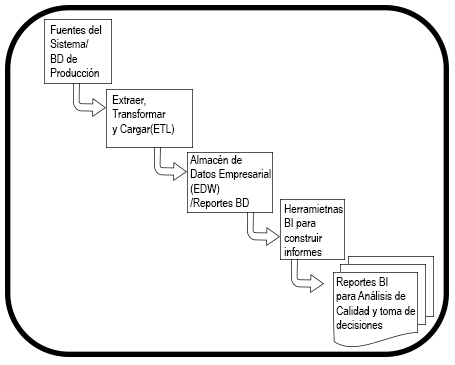
\includegraphics[width=160mm]{Business-Intelligence-stages-as-data-quality-sources-esp.png}
\caption{Etapas de BI como fuentes de datos de calidad}
\label{fig:EtapasDeBiComoFuentesDeDatosDeCalidad}
\end{figure}}
\noindent
Una cuesti�n fundamental es el hecho que una organizaci�n corre sobre datos; y act�a como insumo para el motor de la industria corporativa. Una organizaci�n no puede comprender a sus clientes, proveedores, competidores o a su propia gente, procesos, y rendimiento sin datos de buena calidad. Por consiguiente, la alta direcci�n de una empresa y el �rea de TI (tecnolog�a de la informaci�n) deber�an trabajar juntos para asegurar datos de alta calidad  \cite{eckerson2009ensures}.

\subsubsection{Componentes de BI}

\paragraph{OLAP}\hspace{0pt} \\ \indent
Se refiere al mecanismo por el cual los usuarios de una organizaci�n pueden explorar y realizar cortes de datos, usando herramientas sofisticadas que permiten la navegaci�n de dimensiones tales como el tiempo o jerarqu�as. OLAP, provee vistas resumidas multidimensionales de datos del negocio de una organizaci�n, y es usado para reportes, an�lisis, modelado y planificaci�n para la optimizaci�n de una organizaci�n.\cite{malhotra2001information}\\
Las t�cnicas y herramientas OLAP pueden ser usados para trabajar con datawarehouse o con data marts (un subconjunto de datos de un �rea espec�fica) dise�ados para sistemas sofisticados. Este tipo de consultas son requeridas para descubrir tendencias y analizar factores cr�ticos. Los reportes generan vistas agregadas de datos para mantener la gesti�n informada sobre el estado de sus negocios. Otras herramientas de BI son usadas para almacenar y analizar datos, tales como la miner�a de datos y el datawarehouse; sistemas de soporte o apoyo a las decisiones y previsiones; almac�n de documentos y gesti�n de documentos; gesti�n del conocimiento; mapeamiento, visualizaci�n de informaci�n y paneles (dashboards); sistemas de informaci�n de gesti�n, sistemas de informaci�n geogr�ficas; an�lisis de tendencias; Software como servicio (SaaS) y otros.\cite{malhotra2001information}

\paragraph{An�lisis Avanzado}\hspace{0pt} \\ \indent
Conocido como miner�a de datos y an�lisis predictivos, toma las ventajas de las t�cnicas de an�lisis estad�sticos para predecir o proveer medidas de certeza sobre ciertos hechos.  La gesti�n sobre el rendimiento de una organizaci�n (Portales, cuadros de mando, paneles de control): esta categor�a general normalmente provee un sistema de varios componentes interconectados, de tal forma que en conjunto describan una historia. Por ejemplo, un cuadro de mando integral que muestre componentes de indicadores financieros, todos ellos combinados pueden describir m�tricas y patrones de aprendizaje y crecimiento en las organizaciones.\cite{gangadharan2004business}


\paragraph{BI en tiempo real}\hspace{0pt} \\ \indent
Permite la distribuci�n de m�tricas en tiempo real a trav�s de emails, sistemas de mensajer�a instant�nea y/o pantallas interactivas. 

\paragraph{Datawarehouse y Datamarts}\hspace{0pt} \\ \indent
El datawarehouse es un componente importante de BI. El datawarehouse soporta la propagaci�n f�sica de los datos manejando grandes vol�menes de registros de las organizaciones para integraci�n, limpieza,  agregaci�n y tareas de consulta.\cite{gangadharan2004business}\\
Tambi�n puede contener datos operacionales, los cuales pueden ser definidos como un conjunto actualizable de datos integrados disponibles para toda una organizaci�n, para la toma de decisiones t�cticas de un asunto espec�fico. Contiene datos vivos actualizados en tiempo real, no solamente fotos de un momento espec�fico, y tambi�n conserva un historial m�nimo. Las fuentes de datos pueden ser bases de datos operacionales, datos hist�ricos, datos externos, por ejemplo, de organizaciones de investigaci�n de mercados o desde internet mismo, o informaci�n desde un entorno de datawarehouse ya existente. Las fuentes de datos pueden ser de bases de datos relacionales o cualquier otra estructura que apoya o soporta el conjunto de sistemas transaccionales de una organizaci�n. \cite{gangadharan2004business}\\
Un datamart, tal como se describe en  \cite{kumari2013business}, es una colecci�n de disciplinas organizadas para el apoyo de las decisiones basadas en las necesidades de un departamento dado. Finanzas tiene su data marts, marketing tiene el suyo, y ventas tienen la suya y as� sucesivamente.\\
Cada departamento tiene su propia interpretaci�n de c�mo debe verse un data mart y el data mart de cada departamento es particular y atiende las necesidades espec�ficas del �rea. Similar al datawarehouse, los data marts contienen datos transaccionales que ayudan a expertos en negocios a crear una estrategia basada en el an�lisis de las tendencias y experiencias pasadas. La principal diferencia es que la creaci�n de los data marts se basa en una necesidad espec�fica, predefinida para un grupo determinado. Un data mart puede apoyar o soportar procesos o unidades de negocio espec�ficos \cite{ranjan2009business}.\\
Las herramientas de BI son ampliamente aceptadas como una capa intermedia entre aplicaciones transaccionales y aplicaciones de apoyo a la toma de decisi�n, �stas est�n desacopladas y extraen informaciones de transacciones de negocio. Las habilidades de BI incluyen, apoyo a la decisi�n, procesamiento anal�tico en l�nea, an�lisis estad�sticos,  an�lisis predictivo, y la miner�a de datos \cite{ranjan2009business}.\\
Las fuentes de datos pueden ser bases de datos operacionales, datos hist�ricos, datos externos por ejemplo, desde las empresas de investigaci�n de mercados o desde internet, datos no estructurados de redes sociales, o informaci�n desde un datawarehouse existente. Las fuentes de datos pueden ser bases de datos relacionales o cualquier otra estructura de datos de sistemas transaccionales. Ellos tambi�n pueden residir en muchas plataformas diferentes, tales como tablas, hojas de c�lculo, o informaci�n no estructurada, tales como archivos de texto plano o im�genes y otras informaciones multimedia \cite{ranjan2009business}.\\

\subsubsection{Beneficios de BI}

BI provee muchos beneficios a las compa��as que lo utilizan. Puede ayudar a eliminar muchas conjeturas err�neas dentro de una organizaci�n, mejorando la comunicaci�n entre departamentos mientras se coordinan las actividades, y apoyan a las organizaciones para responder r�pidamente a cambios de condiciones financieras o preferencias de clientes. BI puede ayudar a mejorar el rendimiento general de una organizaci�n \cite{ranjan2009business}.\\
La informaci�n es frecuentemente considerada como el segundo recurso m�s importante que una compa��a tiene (lo m�s valorable de una compa��a son las personas). Cuando una compa��a puede tomar decisiones basadas en informaci�n oportuna y precisa, puede ayudar a mejorar su rendimiento en su segmento de mercado. BI tambi�n agiliza la toma de decisiones, ayuda a actuar r�pida y correctamente con la informaci�n adecuada antes de otras empresas de la competencia. Tambi�n pueden mejorar la experiencia del cliente, teniendo en cuenta la respuesta oportuna y adecuada a los problemas y prioridades de los mismos. A continuaci�n se listan algunos de estos beneficios: 

\begin{itemize}[noitemsep, nolistsep]
\item   Con herramientas de BI, los empleados pueden f�cilmente convertir sus conocimientos de negocio en inteligencia anal�tica para resolver muchas cuestiones de negocio, tales como incrementar la tasa de respuestas desde correos electr�nicos, tel�fonos, y mejorar las campa�as de ventas desde internet.

\item   Con BI, las empresas pueden identificar sus clientes m�s rentables y las razones subyacentes para la lealtad de esos clientes, as� como identificar clientes futuros con grandes potenciales.

\item  Analizar los datos de clics para mejorar las estrategias de comercio electr�nico.

\item  Detecci�n r�pidamente de problemas reportados de productos para minimizar el impacto de las deficiencias en sus dise�os.

\item   Descubrir lavado de dinero de actividades delictivas.

\item  Analizar la rentabilidad potencial del cliente, y reducir el riesgo a trav�s de una puntuaci�n m�s precisa de cr�dito financiero de los mismos.

\item  Determinar cuales son las combinaciones de productos y servicios que los clientes son m�s propensos a comprar y cuando.

\item  Analizar los ensayos cl�nicos de f�rmacos experimentales.

\item  Establecer tarifas m�s rentables para las primas de seguros.

\item  Reducir el tiempo fuera de un equipamiento mediante la aplicaci�n de mantenimiento predictivo.

\item  Determinar con el an�lisis de deserci�n y rotaci�n de clientes, la causa por la cual los clientes se van a los competidores o se convierten en nuestros clientes. 

\item Detectar y disuadir comportamientos fraudulentos, por ejemplo, de picos de uso cuando las tarjetas de  cr�dito o tarjetas telef�nicas son robadas.

\item Identificar nuevos compuestos de f�rmacos moleculares prometedores. 
\end{itemize}



\subsubsection{Tecnolog�a de BI}

La inteligencia empresarial provee datos organizacionales de tal manera que los filtros de conocimientos organizacionales puedan f�cilmente asociarse con estos datos y volverlos en informaci�n para la organizaci�n. Las personas involucradas en procesos de inteligencia de negocios podr�an usar software y otras tecnolog�as para reunir, almacenar, analizar, proveer accesos a datos, y presentar esos datos de una manera simple y �til.\\
El software ayuda en la  gesti�n de una organizaci�n, y a las personas a hacer mejores decisiones de negocios, teniendo la informaci�n precisa, actualizada, y relevante cuando lo necesiten. Algunas empresas usan data warehouse porque es un conjunto de informaci�n l�gica recolectado desde varias bases de datos operacionales con el objetivo de crear inteligencia de negocios \cite{ranjan2009business}.\\
Para que los sistemas BI trabajen efectivamente, existen algunas restricciones t�cnicas que deber�an ser tratadas: 

\begin{itemize}[noitemsep, nolistsep]
\item Seguridad y acceso de usuarios al data warehouse.
\item Volumen de datos (capacidad).
\item Cu�nto tiempo ser� almacenado el dato (retenci�n de datos).
\item Sizing y rendimiento de infraestructura (servidores).
\end{itemize}

\noindent
Las personas que trabajan en BI desarrollan productos que facilitan el trabajo, especialmente cuando las tareas de inteligencia involucran conseguir y analizar grandes cantidades de datos no estructurados. Cada proveedor t�picamente define BI de una forma particular,  y comercializa herramientas para hacer BI de la forma en que cada uno lo propone. BI incluye herramientas en diversas categor�as, incluyendo las siguientes: \cite{ranjan2009business}.

\begin{itemize}[noitemsep, nolistsep]
\item  AQL (Associative Query Logic) -  L�gica Asociativa de Consultas.
\item  M�tricas y mediciones del rendimiento del negocio.
\item Planeamiento Empresarial.
\item Data mining (DM), Data Farming, y Data warehouses.
\item Sistemas de apoyo a la decisi�n (DSS) y predicci�n.
\item Datawarehouse de documentos y gesti�n documental.
\item Sistema de Gesti�n Empresarial.
\item Finanzas y presupuestos.
\item Recursos humanos.
\item Gesti�n del conocimiento.
\item Mapeamiento, visualizaci�n de la informaci�n, y paneles de control (dashboards).
\item Sistemas de gesti�n de informaciones.
\item Sistemas de informaci�n geogr�fica (GIS).
\item OLAP (Online Analytical Processing) y an�lisis multidimensional; a veces simplemente llamado ``Analytics`` (basado tambi�n en ``hipercubo`` o ``cubo``).
\item BI en tiempo real.
\item An�lisis de datos estad�sticos y t�cnicos.
\item Gesti�n de la l�nea de producci�n, Gesti�n de demandas.
\item Gesti�n de la cadena de Suministro/Gesti�n de la cadena de demanda.
\item An�lisis de tendencias.
\item Reportes y consultas de usuarios/usuarios-finales.
\end{itemize}


\noindent
BI frecuentemente usa indicadores de rendimientos (KPIs, key performance indicators) para evaluar el estado actual de los negocios y para establecer un plan de acci�n. M�s y m�s organizaciones han comenzado a disponibilizar m�s datos con mayor velocidad. En el pasado, los datos s�lo estaban disponibles despu�s de uno o dos meses, lo que no ayudaba a los directivos de empresas para ajustar las actividades con la velocidad necesaria para alcanzar sus objetivos. Recientemente, los bancos han intentado disponibilizar los datos en el intervalo m�s corto y reduciendo los atrasos \cite{ranjan2009business}.\\
Por ejemplo, para negocios de alto riesgo operacional (por ejemplo, tarjetas de cr�ditos), un banco multinacional disponibiliza los datos relacionados con KPI semanalmente, y en ocasiones ofrece un an�lisis diario de los n�meros. Esto significa que los datos normalmente est�n disponibles  a cada 24 horas, requiriendo la automatizaci�n y el uso de sistemas de TI.

\subsubsection{Breve discuci�n}

La experiencia actual de cualquier nueva forma de organizaci�n es la cadena de valor, la cual es un conjunto de actividades primarias y secundarias que crea valor para los clientes. \cite{denison1997toward} examina muchas actividades cr�ticas relacionada a la cadena de valor. Sin un BI eficaz para dirigir las organizaciones orientadas a los procesos de apoyo, esto no ser�a posible.\\
\cite{davenport1993process} describe varias cuestiones en la reingenier�a en las innovaciones de los procesos de negocio. De acuerdo a \cite{adelman2002found}, BI es un t�rmino que engloba un amplio rango de software de an�lisis y soluciones para recolectar, consolidar, analizar y proveer acceso a la informaci�n de una manera sencilla para que los usuarios de una empresa puedan tomar mejores decisiones de negocio. \cite{malhotra2001information} describe a BI como un facilitador de conexiones en una nueva forma de organizaci�n, trayendo informaci�n en tiempo real para centralizar repositorios y apoyar el analisis, que puede ser explotada en cada nivel horizontal y vertical, dentro y fuera de la empresa.\\
Bi describe el resultado de un an�lisis profundo de los datos detallados del negocio, incluyendo base de datos y tecnolog�as de aplicaci�n, as� como pr�cticas de an�lisis \cite{gangadharan2004business}. BI es t�cnicamente m�s amplio, lo que potencialmente engloba la gesti�n del conocimiento, la planificaci�n de recursos empresariales, sistemas de apoyo a la toma de decisiones y la miner�a de datos  \cite{gangadharan2004business}.\\
\cite{nguyen2005sense} introdujeron una arquitectura mejorada de BI que cubre un proceso completo para identificar, interpretar, predecir, automatizar y responder a los ambientes de negocios; y por lo tanto tiene como objetivo reducir el tiempo de reacci�n necesario para las decisiones empresariales. \cite{nguyen2005sense} propone una infraestructura de TI basada en eventos para operar aplicaciones de BI que permiten an�lisis en tiempo real a trav�s de procesos de negocios corporativos, y brindar recomendaciones autom�ticamente para optimizar las operaciones comerciales, y cerrando efectivamente la brecha entre sistemas de BI y procesos de negocio.\\
\cite{seufert2005enhanced} sugieren una arquitectura de BI mejorada, que tiene como objetivo aumentar el valor de la informaci�n mediante la reducci�n del tiempo de acci�n y la interconexi�n de los procesos de negocio en la toma de decisiones.\\
Las empresas no solo desean conocer lo que ha sucedido, sino necesitan saber las causas subyacentes. Por ejemplo, en lugar de saber cu�ntas mantas fueron vendidas en un mes, las empresas desean entender cu�ntas fueron vendidas en un pa�s determinado durante un evento meteorol�gico. BI proporciona una visi�n integrada unificada de las actividades empresariales. Las empresas han construido sistemas de BI que apoyan an�lisis de negocio y de toma de decisiones para ayudarlos a un mejor entendimiento de sus operaciones y competir en el mercado \cite{gangadharan2004business}.\\
Algunas innovaciones en tecnolog�as de almacenamiento de datos est�n superando significativamente el progreso en potencia de procesamiento \gls{sig:CPU}, anunciando una nueva era para BI en tiempo real. Como resultado, algunos proveedores de software con herramientas superiores ofrecen una suite completa de aplicaciones para an�lisis de BI,  herramientas y modelos de datos que permiten a una organizaci�n aprovechar su informaci�n. Las herramientas BI facilitan el acceso a un gran volumen de datos corporativos, y convertir esos datos en informaci�n �til y procesable que sea consistente a trav�s de la versi�n coherente de la verdad.\\
Las empresas a�n sienten que BI tiene complejidades relacionadas con la tecnolog�a y que puede usarse solamente por especialistas con conocimientos t�cnicos, adem�s que los costos de implantaci�n son altos. Las empresas requieren estos an�lisis en tiempo real para los proyectos a corto plazo. El BI tradicional puede que no haga esto, pero en un ambiente BI en tiempo real ciertamente podr�a atender las necesidades actuales de las empresas. Los datos finalmente son considerados como recursos corporativos en una nueva disciplina. Cualquier sistema transaccional (incluyendo \gls{sig:ERP} y \gls{sig:CRM}) y cualquier aplicaci�n de apoyo a la decisi�n (incluyendo data warehouses y data marts) son BI, si y s�lo si fueron desarrollados bajo la protecci�n y la metodolog�a de una iniciativa estrat�gica de toda la Organizaci�n \cite{gangadharan2004business}.\\
Los sistemas tradicionales de BI consisten en una base de datos en el back-end, una interfaz de usuario en el front-end, software que procesa la informaci�n para producir la propia inteligencia de negocios, y un sistema de informes. Las capacidades de BI incluyen apoyo a la decisi�n, procesamiento anal�tico en linea, an�lisis estad�sticos,  predicci�n y miner�a de datos.\\
Diferentes sectores como fabricantes, comercios electr�nicos, empresas de telecomunicaciones, aerol�neas, minoristas, sistemas de salud, servicios financieros, bioinform�tica y hoteles utilizan BI para apoyo a clientes, investigaci�n de mercado, segmentaci�n, rentabilidad del producto, an�lisis y distribuci�n de stock, an�lisis estad�stico, informes multidimensionales, detecci�n fraudes, entre otros.\\
BI y miner�a de datos es un �rea que est� fuertemente influenciado por t�cnicas estad�sticas tradicionales, y la mayor�a de los m�todos de miner�a de datos revela una fuerte base de m�todos estad�sticos y de an�lisis de datos. Algunas de las t�cnicas tradicionales de miner�a de datos incluyen clasificaci�n, agrupaci�n, an�lisis de valores at�picos, patrones secuenciales, an�lisis de series temporales, la predicci�n, la regresi�n, an�lisis de enlaces (asociaciones),  y m�todos multidimensionales incluyendo el procesamiento anal�tico en l�nea \gls{sig:OLAP}. Estos pueden clasificarse en una serie de t�cnicas de miner�a de datos, que se clasifican e ilustran en la Tabla 1 \cite{goebel1999survey}.

%\textsc{\begin{figure}[!htb]
%	\centering
%	
\includegraphics[width=160mm]{insight-bi.png}
%	\caption{Representaci�n de un dashboard \gls{sig:BI}}
%	\label{fig:BI}
%\end{figure}}

%\vspace*{2\baselineskip}
\newlength\q
\setlength\q{\dimexpr .5\textwidth -2\tabcolsep}
\begin{table}[H]
\begin{tabular}{|p{\q}|p{\q}|}
\hline
T�CNICAS & DESCRIPCI�N\\ \hline
Modelo predictivo & Predecir valor para un atributo espec�fico del elemento de datos.\\ \hline
Caracterizaci�n y miner�a de datos descriptivo &
Distribuci�n, dispersi�n y excepci�n de datos\\ \hline
Asociaci�n, correlaci�n, an�lisis de la causalidad (An�lisis Link) &
Identificar relaci�n entre atributos\\ \hline
Clasificaci�n &
Determinar a qu� clase pertenece un elemento de datos\\ \hline
La agrupaci�n y an�lisis de valores at�picos  &
Partici�n de un conjunto en clases, con lo cual elementos con caracter�sticas similares se agrupan\\ \hline
An�lisis de patrones temporal y secuencial &
Tendencia y desviaci�n, patrones secuenciales, frecuencia\\ \hline
OLAP(Procesamiento Analitico en Linea) &
Herramientas OLAP permiten a los usuarios analizar distintas dimensiones de datos multidimensionales. Por ejemplo, proporciona series temporales y puntos de vista de an�lisis de tendencias.\\ \hline
Modelo de visualizaci�n &
Hacer f�cil la descubierta de conocimiento usando charts, plots, histograms y otros medios visuales\\ \hline
An�lisis Exploratorio de Datos(EDA) &
Explorar un conjunto de datos sin una fuerte dependencia en hip�tesis o modelos; el objetivo es identificar patrones de una manera exploratoria\\ \hline

\end{tabular}
\caption{T�cnicas actuales de BI}
\label{tab:tecnicasActualesBI}
\end{table}

\noindent
En el siguiente cap�tulo se presenta una introducci�n a los m�todos y t�cnicas de an�lisis exploratorio, y en especial la t�cnica actualmente llamada Data Discovery, la cual fue aplicada en este trabajo.

\subsection{Data Discovery  Analysis}
Data discovery es una arquitectura de BI destinado a informes interactivos y en tiempo real que pueden ser explorados desde m�ltiples or�genes\cite{marakas2003modern}.
La mayor parte de la base instalada en todo BI son propietarias de empresas tradicionales que han construido sus plataformas alrededor de una capa sem�ntica y metadatos, la cual es generalmente accesible solo por herramientas del propio fabricante. La situaci�n actual de car�cter propietario de la capa sem�ntica tradicional de BI fue aceptada y adoptada por m�s organizaciones como un facilitador para an�lisis "ad hoc" a cambio de una �nica y confiable versi�n de la realidad, que puede ser accedida f�cilmente por los usuarios de negocio, ocultando los aspectos t�cnicos y la complejidad de las estructuras de datos subyacentes. Sin embargo, con la adopci�n y r�pido crecimiento de las herramientas de data discovery como Qlik, Tableau, y Tibco Spotfire, los usuarios buscan cada vez m�s acceso a datos confiables en capas sem�nticas cerradas, y los proveedores de BI se enfrentan a un reto dif�cil para seguir siendo relevantes en un mercado que est� en transici�n. La respuesta de los proveedores tradicionales y la inversi�n significativa hasta la fecha, ha sido la utilizaci�n de sus capas sem�nticas existentes para promover la gesti�n a nivel empresarial de sus propias herramientas de data discovery desarrolladas internamente. Esto ha sido un mecanismo para diferenciar sus soluciones de las de proveedores de data discovery pure-play. Mientras que, en teor�a, este enfoque logra un equilibrio entre la facilidad de uso y escalabilidad empresarial. Esto ha mostrado poco �xito para la mayor�a de los proveedores de BI tradicionales como huecos de importantes funcionalidades que permanecen entre sus herramientas de data discovery desarrolladas internamente y los de los proveedores especialistas de data discovery.\cite{parenteau2015rise}\\
La capa sem�ntica que sirve como la base de la mayor�a de las plataformas BI tradicionales ha sido ampliamente adoptada por muchas organizaciones a trav�s de los a�os y ha sido promovida y generalmente aceptada como un componente esencial de una plataforma BI.  Proveedores como SAP (BusinessOjects), IBM (Cognos) u Oracle (OBIEE) mantienen una gran base instalada de clientes que han invertido mucho en el desarrollo, operaci�n y mejora de estas plataformas construidas alrededor de una definida y centralizada capa sem�ntica propietaria.\\
Este enfoque ha funcionado bien cuando el objetivo fuera una �nica fuente de datos, en apoyo a sistemas definidos de registros centralizados de informes y gesti�n de dashboards fomentando la consistencia, la gobernanza e integraci�n entre las plataformas de presentaci�n y capas de metadatos. Sin embargo, con el surgimiento y expansi�n de data discovery, el concepto de auto servicio cobr� preponderancia. Los usuarios de negocio y an�lisis ahora tienen acceso a un gran rango de herramientas que promueven y apoyan el uso aut�nomo sin la participaci�n de TI. Como tal, hay una necesidad emergente para acceder a las reglas de negocio integradas dentro de la capa sem�ntica propietaria de herramientas de BI existentes.\\
Mientras esto no es posible a�n en la mayor�a de los casos hoy en d�a, algunos proveedores ya han comenzado a adoptar un enfoque cada vez m�s abierto para sus capas sem�nticas propietarias, y esto puede llevar a un cambio mayor de mercado con el tiempo. La oportunidad probablemente ser� dictada por el �xito que los proveedores tradicionales de BI tengan con el desarrollo y la adopci�n de sus propias ofertas de data discovery, que se ha limitado hasta la fecha.\\
El acceso abierto a metadatos no es in�dito en BI y en mercados analiticos. Ejemplos incluyen Oracle OBI EE, Microsoft Power, SAP BusinessObjects y, m�s recientemente, conectividad nativa de Tableau para modelo de datos Birst a trav�s de su capa sem�ntica propietaria.\\
Oracle BI Enterprise Edition(OBI EE) fue uno de los primeros productos de plataformas BI para tener una capa sem�ntica abierta, un vestigio de los or�genes del producto como una nueva plataforma web abierta, desarrollada por nQuire, posteriormente adquirida por Siebel en 2001, y finalmente por Oracle en el 2005. Con OBI EE, el modelo de datos puede ser publicado y accedido con una conexi�n ODBC que puede ser consumida por herramientas e interfaces de terceros. Inicialmente, esto es c�mo Oracle proporciona conectividad a su herramienta interna de informes de producci�n desarrollada, Oracle BI Publisher. M�s all� de eso, pocos clientes son conscientes de esta capacidad, y citan los malos resultados como una raz�n por la que no fue adoptado ampliamente.\\
La reciente alianza entre Birst y Tableau, establecida en Abril 2015, es el m�s reciente ejemplo de este cambio hacia acceso abierto e integraci�n entre proveedores puros de data discovery y fabricantes tradicionales de BI. Antes del anuncio, Birst no hab�a permitido el acceso a su estructura de datos propietaria o capa sem�ntica, hizo accesible s�lo a de informes, dashboard y capacidades data discovery auto-contenidas dentro de la cartera Birst. A trav�s de la alianza y desarrollo conjunto, se a�adi� una conexi�n con Tableau que permite la conexi�n directa con el medio ambiente Birst. Esto proporciona una mayor flexibilidad y una gama m�s amplia de opciones a los clientes comunes.\\
Una alianza similar a la que existe entre Birst y Tableau fue anunciada en 2014 entre SAP y Microsoft permite a los usuarios Power Query acceder a la capa sem�ntica de SAP BusinessObjects (Universe). Este acuerdo permite a los clientes comunes la opci�n de usar herramientas de Microsoft Power BI para data discovery a la vez aprovechan las inversiones en el SAP BusinessObjects Universe.\\
Un inconveniente de estas alianzas es que son actualmente unidireccionales en su naturaleza y s�lo otorgan acceso de s�lo lectura a herramientas de data discovery de otros proveedores de BI a la capa sem�ntica propietaria de proveedores de BI tradicionales. Como tal, ellos todav�a no apoyan la promoci�n de modelos de datos derivados de herramientas de data discovery en la capa sem�ntica como una forma de promover a proveedores independientes que rigen capacidades de data discovery. Esto es, sin embargo, una oportunidad potencial de modernizaci�n que los proveedores tradicionales pueden considerar.\\
Proveedores de software independientes e integradores de sistemas desarrollar�n nuevas soluciones de capa intermedia que facilitan el acceso a la capa sem�ntica a las herramientas de data discovery a trav�s de servicios web.\\
Mientras que los clientes prefieren una �nica soluci�n de sus proveedores titulares, ya sea de los proveedores de plataforma tradicional de BI o de proveedor de data discovery, los clientes actualmente encontrar�n m�s oportunidades para acceder a la capa sem�ntica desde los integradores de software y los proveedores independientes menores.
\subsection{Framework de An�lisis de Negocio de Gartner}
En este trabajo fue adoptado un Framework de An�lisis de Negocio de Gartner, el cual se describe a continuaci�n. 

Hay una serie de defectos relacionados en la mayor�a de las organizaciones con relaci�n a BI y plataformas analiticas, as� como una percepci�n err�nea de sus objetivos y c�mo gestionarlos. Los equipos de BI, especialmente si se encuentran en el �rea de TI, creen que:

\begin{itemize}[noitemsep, nolistsep]

\item La plataforma anal�tica de negocio debe ser una soluci�n estrechamente integrada con pocos componentes, preferentemente de un �nico proveedor, para entregar una sola versi�n de la verdad para la organizaci�n.

\item La informaci�n puede ser confiable s�lo si est� almacenada en un data warehouse corporativo y entregada a los consumidores de informaci�n usando artefactos de BI, tales como informes y dashboards.

\item Las informaciones creadas  o manipuladas por los usuarios de negocios inevitablemente producir�n discrepancias a trav�s de diferentes an�lisis, lo que lleva a decisiones equivocadas,  generando caos en la organizaci�n a trav�s del tiempo.

\item La responsabilidad del departamento TI para la gesti�n de informaci�n termina en la capa sem�ntica de BI y en los contenidos orientados a TI. 

\item Procesos anal�ticos orientados al negocio est�n fuera del alcance y no soportados por TI.
Hay varios problemas orientados a la informaci�n documentados en el mundo BI y an�lisis, que obligan a los l�deres de BI a seguir estas creencias y desplegar un entorno de BI centralizado y monol�tico, que termina siendo impuesta a los usuarios, independientemente de su adecuaci�n a las necesidades. 

\item Los proveedores licenciados de BI, a favor de sus propias plataformas, apoyan este enfoque.

Seg�n Gartner, una plataforma anal�tica necesitan evolucionar m�s all� del pensamiento monol�tico. Debe ocurrir una transformaci�n para ofrecer diferentes soluciones para las diferentes necesidades del usuario, con un conjunto diverso de niveles de integraci�n, y encontrar un equilibrio entre confianza y agilidad. El prop�sito es ayudar a los usuarios a alcanzar sus objetivos de negocio a trav�s del uso de la tecnolog�a apropiada, no para erradicar las soluciones de BI orientados al usuario que resuelven parcialmente sus problemas de hoy.

El entorno de BI y el an�lisis resultante tambi�n exigir� cambios en los procesos de gesti�n de la informaci�n, como atribuir nuevas responsabilidades a diferentes personas en la organizaci�n.

\end{itemize}

A continuaci�n el framework de an�lisis de negocios.
La figura ~\ref{fig:FrameworkAnaliticoNegociosGartner} presenta el framework de an�lisis de negocios de Gartner. 

\textsc{\begin{figure}[H]
\centering
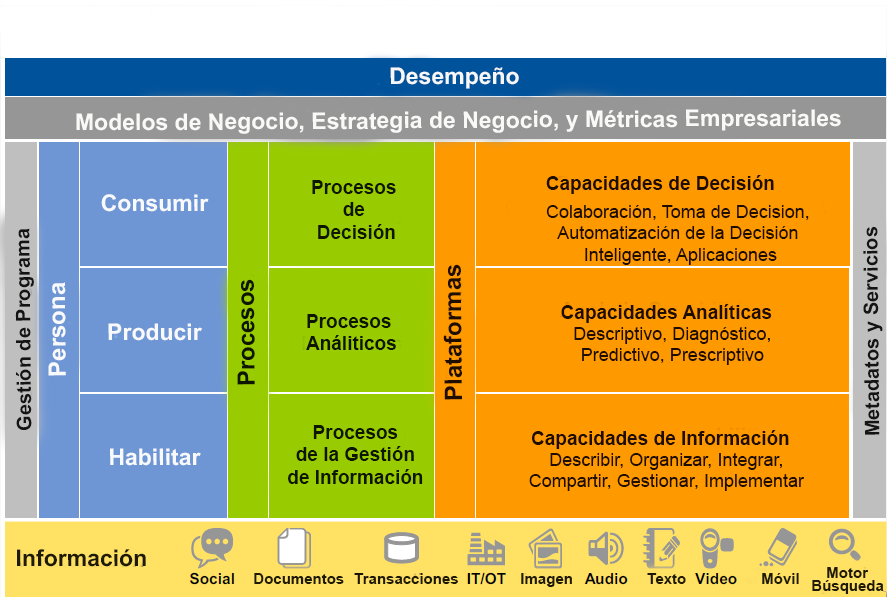
\includegraphics[width=160mm]{Framework-Analitico-de-Negocios-Gartner.png}
\caption{Framework Analitico de Negocios Gartner}
\label{fig:FrameworkAnaliticoNegociosGartner}
\end{figure}}

El framework de an�lisis de Gartner identifica las personas, los procesos y componentes de la plataforma que apoyan la transformaci�n de la informaci�n en un mejor rendimiento de la organizaci�n. El uso de esta herramienta est� hecha por la lectura desde arriba hacia abajo, comenzando con los resultados del negocio y luego descifrando las composiciones anal�ticas de apoyo y la informaci�n necesaria para alcanzarlos. De acuerdo a las necesidades de los usuarios, la plataforma debe ser redise�ada con un amplio conjunto de capacidades t�cnicas (llenando los vac�os), nuevas responsabilidades y organizaci�n. Centr�ndose en las herramientas o normalizaci�n de proveedor  por s� sola no es la respuesta.

El framework es tambi�n muy �til para definir los estados actuales y futuros de la arquitectura. La diferencia entre ellos es el mapa de rutas e incluye cambios en personas y procesos.  La organizaci�n muy probablemente tambi�n necesitar� re-organizar y capacitar a los proveedores y usuarios de BI y an�lisis.
Los usuarios de negocio deben ganar acceso a las herramientas anal�ticas  adecuadas, de acuerdo a sus metas y habilidades, y un rango comprensivo de fuente de datos con tipos de datos variados, granularidad adecuada y accesos apropiados.
Teniendo en cuenta el espectro de capacidades anal�ticas con �nfasis en las plataformas, en particular, el componente de capacidad anal�tica, podemos notar cuatro estilos anal�ticos que se detalladan a continuaci�n  (Figura~\ref{fig:espectroAnalitico}).

\textsc{\begin{figure}[H]
\centering
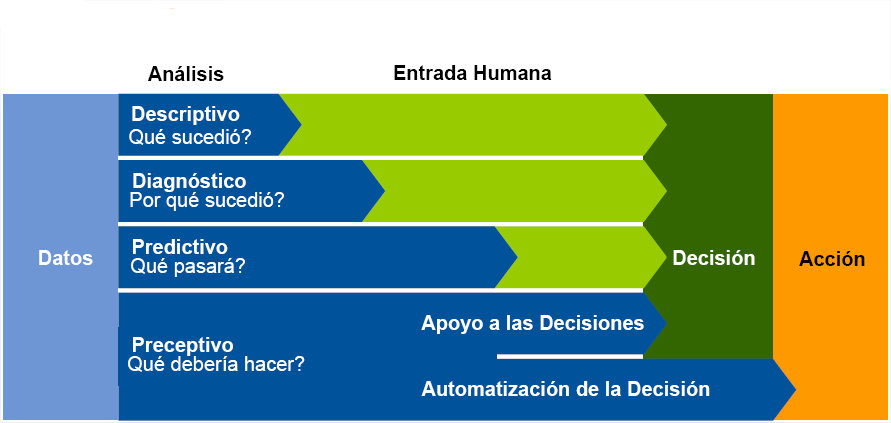
\includegraphics[width=160mm]{Espectro-Analitico.png}
\caption{Espectro Analitico}
\label{fig:espectroAnalitico}
\end{figure}}

Las capacidades anal�ticas implementadas en organizaciones son a menudo limitadas el an�lisis descriptivo, a trav�s de reportes b�sicos y dashboards. Con esto, la pregunta, ``Qu� paso\mbox{?}`` puede ser respondida. Despu�s de conocer ``Que,`` , lo m�s probable es que los usuarios tambi�n pregunten, ``Por qu� pas�\mbox{?}``.  Abordar adecuadamente esto requiere mucha m�s agilidad y m�s capacidades avanzadas de exploraci�n de la informaci�n. Despliegues de BI tradicionales tienden a tener huecos en esta �rea, pero TI por lo general pasa por alto el impacto de esta problem�tica y contin�a impulsando el est�ndar del proveedor y sus herramientas no aptas-para-prop�sito. Como consecuencia, los usuarios recurrir�n a Excel, consultas ad hoc, extracciones de datos y a los equipos de shadow TI para lograr sus metas de an�lisis. 


Los l�deres de BI deben extender el BI y la plataforma anal�tica hasta el an�lisis de diagn�stico para complementar el an�lisis descriptivo. Aqu� es donde OLAP y los modelos de datos en memoria son utilizadas para proporcionar una navegaci�n f�cil y r�pida de datos sin una consulta predefinida. Aprovechando mejoras en el nivel de acceso a datos, tambi�n vemos la necesidad de mejorar las capas sem�nticas abstrayendo la complejidad del modelo f�sico subyacente. Esto puede hacer que sea mucho m�s f�cil para el descubrimiento de autoservicio sin el cuello de botella de TI que se encuentra en un t�pico equipo de BI.

M�s all� de la capa de datos, vemos la introducci�n de nuevas herramientas de visualizaciones de datos, y aqu� es donde el enfoque del r�pido crecimiento de las herramientas de data discovery se concentran. Pero herramientas tradicionales pueden tambi�n proporcionar mejoras con un mayor enfoque en informes m�s comprensivos(como el an�lisis de varianza),  planificaci�n integrada, dashboards y informes KPI.

A trav�s del tiempo, con un crecimiento a un alto  nivel de madurez de an�lisis, la organizaci�n deber�a moverse dentro del an�lisis predictivo y preceptivo. Esto requiere un incremento significante en los niveles de habilidades del analista de negocios. Modelos predictivos requieren desarrollo y mantenimiento con l�gicas complejas y reglas de negocio. Ellos incorporan m�todos sofisticados  que pueden tambi�n requerir un entendimiento profundo de la estad�stica o investigaci�n operacional.

Adem�s, las organizaciones deben darse cuenta de que hay necesidad de mezclar todas estas diferentes t�cnicas en soluciones integrales en lugar de dejarlos aislados.

Redise�ar el BI y la Plataforma Analitica
Los l�deres de BI deben seguir las herramientas fundamentales descritas anteriormente para as� con �xito redise�ar el BI y la plataforma de an�lisis. Gartner recomienda la instalaci�n de una arquitectura por niveles compuesta por:

\begin{itemize}[noitemsep, ]
\item Portal de Informaci�n.
\item Workbench An�litico.
\item Laboratorio de datos cient�ficos.
\end{itemize}

En la figura ~\ref{fig:tipicoUsoEstilosAnaliticos} se presenta la representaci�n de BI en niveles y la plataforma analitica, la cual puede ser utilizada como una gu�a gen�rica que puede ser ajustado de acuerdo a las caracter�sticas espec�ficas de la organizaci�n.


\textsc{\begin{figure}[H]
	\centering
	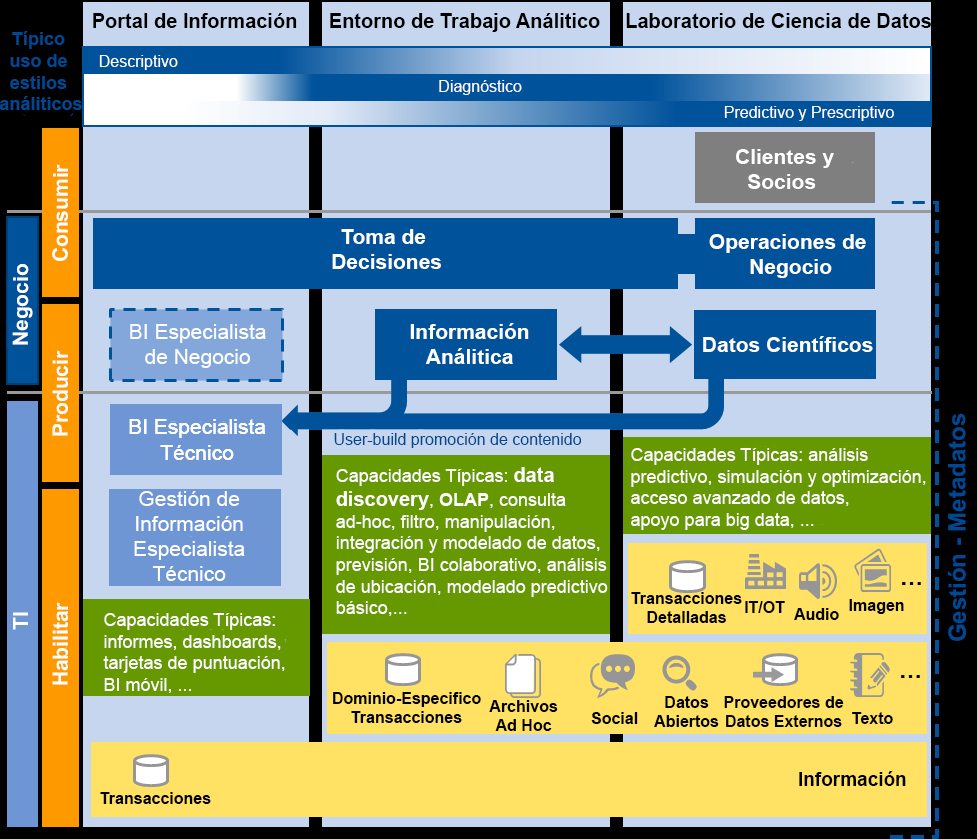
\includegraphics[width=160mm]{Tipico-uso-de-estilos-analiticos.png}
	\caption{Tipico uso de estilos an�liticos}
	\label{fig:tipicoUsoEstilosAnaliticos}
\end{figure}}

Para hacer realidad la visi�n de los tres niveles y ser capaz de maximizar sus fortalezas, los l�deres de BI necesitan implementar nuevas capacidades t�cnicas para proporcionar nuevos estilos de an�lisis, mejorar el uso de las herramientas existentes a trav�s de una mejor integraci�n global, y proporcionar metadatos comunes y gobernanza. Procesos, roles de personas y responsabilidades, son de suma importancia para el �xito. 

Ellos deben ser tratados  en conjunto con la plataforma t�cnica como se describe en el framework de an�lisis de negocios de  Gartner.

Vamos a ampliar cada nivel para entender c�mo integrar y aprovecharlos en conjunto.

\subsubsection{Portal de informaci�n}

Seguir de cerca las caracter�sticas de sistemas de registros desde el Pace Layer Model.
El portal de informaci�n es el �rea de trabajo donde los usuarios de negocio pueden encontrar r�pida y f�cilmente las m�tricas clave de confianza con la cual la organizaci�n mide su rendimiento. Por lo general hecho de capacidades de informes y dashboard que proporciona contenido para los consumidores de informaci�n. Sus productos son el resultado de un proceso de desarrollo formal que abarca que un usuario de negocios establezca requisitos y un especialista t�cnico(t�picamente de TI, pero cada vez m�s de negocio) los implemente.

Capacidades t�picas de la plataforma:
\begin{itemize}[noitemsep, nolistsep]	
	\item Informes.
	\item Dashboards.
	\item Integraci�n Microsoft Office.
	\item BI m�vil.
	\item An�lisis integrada.
\end{itemize}
Ejemplo de herramientas y proveedores:
\begin{itemize}[noitemsep, nolistsep, nosep]
	\item SAP BusinessObjects.
	\item IBM Cognos.
	\item Oracle BI.
	\item Microsoft Reporting Services.
	\item MicroStrategy.
	\item Information Builders WebFocus.
\end{itemize}

\subsubsection{Workbench anal�tico}
El workbench anal�tico es el �rea de trabajo usado para investigar tendencias en indicadores de confianza o detectar patrones en otros conjuntos de datos --- desde m�ltiples fuentes --. que pueden convertirse en oportunidades o riesgos. Es una capa �gil para explorar informaci�n y tener acceso a un amplia gama de fuentes de datos,  con limitado o ning�n apoyo de expertos t�cnicos. Los conjuntos de herramientas deber�an incluir una herramienta de data discovery  (descubrimiento de datos) y un n�mero de otras capacidades para ayudar a los usuarios de negocios a extraer valor de la  informaci�n de forma aut�noma.

En el espectro de an�lisis, el workbench es capaz de proporcionar an�lisis descriptivo ,pero por lo general se centrar� en el an�lisis de diagn�stico. En algunos casos --  es decir, a trav�s del uso de herramientas de data discovery m�s centrado al an�lisis. -- Puede extender a un nivel b�sico de an�lisis predictivo y ganar� el modelado de datos y capacidades anal�ticas m�s avanzadas en el futuro.

Capacidades t�picas de la plataforma:
\begin{itemize}[noitemsep, nolistsep]	
	\item Data discovery.
	\item Informes/consultas Ad hoc.
	\item Inteligencia geoespacial y localizaci�n.
	\item An�lisis integrado avanzado.
	\item OLAP.
	\item Mashup de datos y modelado de usuarios de negocios.
	\item Colaboraci�n.
	\item Filtrado y manipulaci�n de datos.
\end{itemize}

Ejemplo de herramientas y proveedores:
\begin{itemize}[noitemsep, nolistsep]
	\item Tableau Software.
	\item Qlik.
	\item Tibco Spotfire.
	\item SAS Visual Analytics.
	\item SAP Lumira.
	\item Oracle Endeca Information Discovery.
	\item MicroStrategy Visual Insight.
	\item Alteryx.
	\item Microsoft SQL Server Analysis Services and Power BI.
\end{itemize}


\subsubsection {Laboratorio de datos cient�ficos}

El laboratorio cient�fico de datos es el �rea de trabajo donde analisis avanzados se llevan a cabo y es la incubadora ideal para iniciativas big data. Es un entorno flexible donde experimentos de prueba y error es actualmente alentado para generar ideas impactantes para la organizaci�n.

Un amplio conjunto de capacidades t�cnicas es esperado y a menudo proporcionado por herramientas especializadas con integraci�n TI m�nima, destinada a entregar agilidad y capacidad de responder las preguntas imprevisibles. Esto es porque TI tiende a pasar por alto esta �rea a favor de inversi�n en el portal de informaci�n. Los usuarios son cualificados y experimentados, a menudo m�s que los expertos t�cnicos en TI. Sus conjuntos de herramientas incluyen capacidades de data mining, predicciones y otras herramientas de estad�sticas y an�lisis complejos.\\


Capacidades t�picas de la plataforma:
\begin{itemize}[noitemsep, nolistsep, nosep]
	\item Acceso avanzado de datos.
	\item Soporte para fuentes de big data.
	\item An�lisis descriptivo avanzado.
	\item An�lisis predictivo.
	\item Predicci�n.
	\item Optimizaci�n.
	\item Simulaci�n.
	\item Otros an�lisis avanzado.
	\item Aunque no capacidades BI, Hadoop y bases de datos NoSQL tambi�n deben ser referenciados aqu�.
\end{itemize}

%\vspace{-50mm}
Ejemplo de herramientas y proveedores:
%\vspace{-50mm}
\begin{itemize}[noitemsep, nolistsep, nosep]
	\item SAS Enterprise Miner.
	\item IBM SPSS.
	\item SAP InfiniteInsight.
	\item Revolution Analytics y R.
	\item RapidMiner.
	\item Knime.
	\item Alteryx.
	\item FICO.
	\item Dell StatSoft.
	\item Cloudera.
	\item Hortonworks.
	\item MapR y otras distribuciones Hadoop.
\end{itemize}

%\vspace{-50mm}
Entender las caracter�sticas de BI en niveles y la plataforma anal�tica.
La siguiente tabla resume las caracter�sticas que posee cada una de las tres capas. Los l�deres de BI deber�an deber�n intentar entender los huecos en su plataforma anal�tica, y cambiar sus estrategias en consecuencia.

\textsc{\begin{figure}[H]
		%\centering
		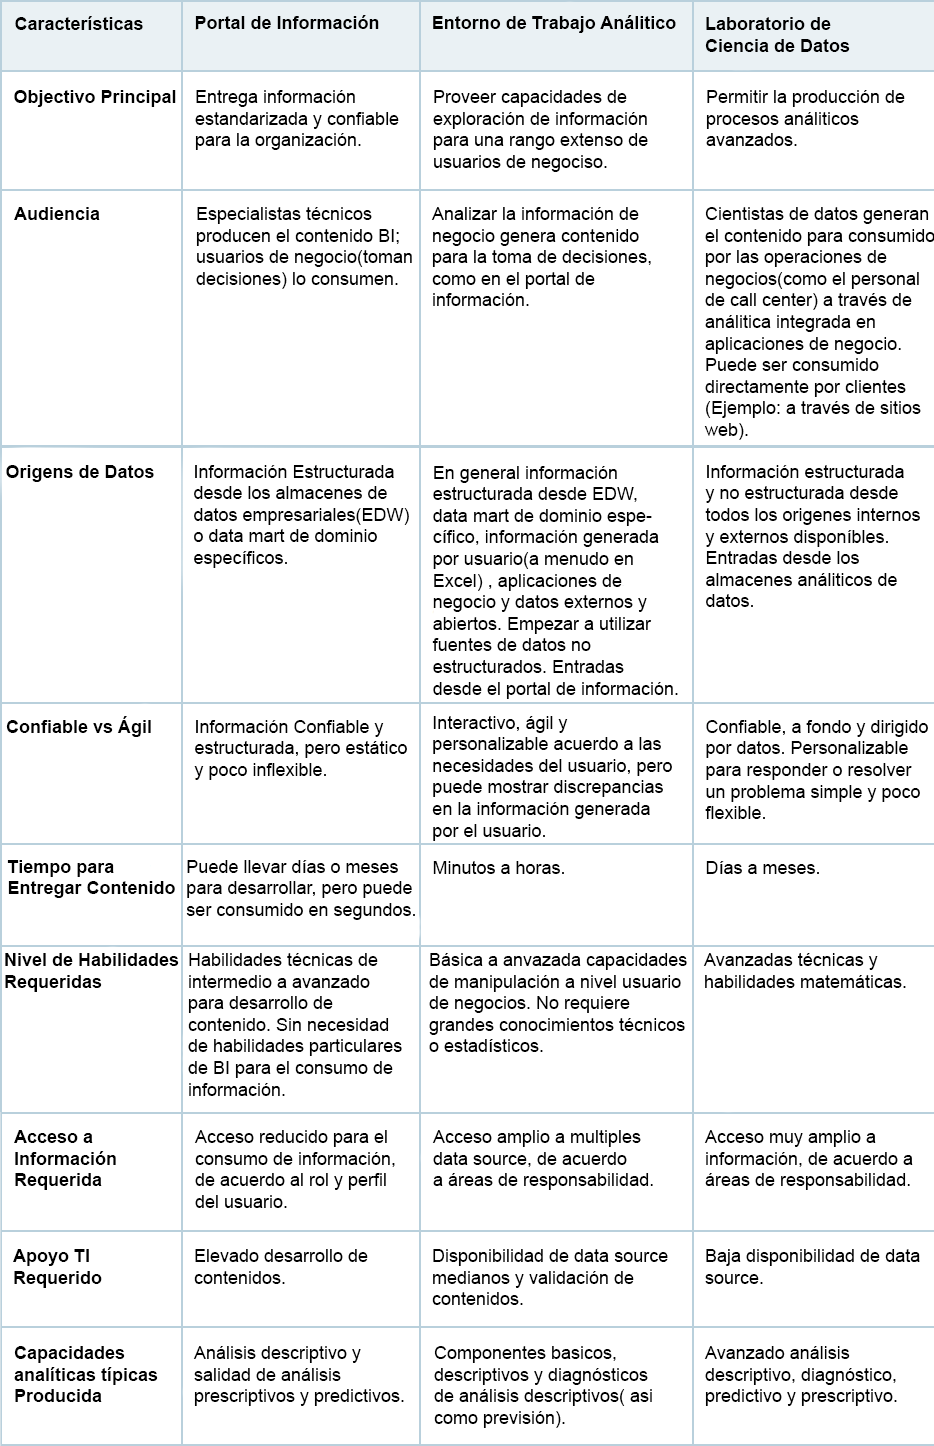
\includegraphics[width=160mm,height=0.9\textheight]{CaracteristicasBiNivelesPlataformaAnalitica.png}
		\caption{Caracter�sticas de BI en niveles y Plataforma Anal�tica}
		\label{fig:caracteristicasBiNivelesPlataformaAnalitica}
	\end{figure}}
		
		
\fontsize{12}{12}\selectfont
\chapter{CAPITULO 3}
%\vspace{-25mm}
\section{Selecci�n de la herramienta para Data Discovery}
%\vspace{-25mm}
Fueron analizados los estudios de Gartner\cite{herschel2015magic}\cite{sallam2015critical} para la selecci�n de la mejor herramienta que se adecue a los criterios necesarios para ser utilizado en esta tesis. Estos documentos realizan un an�lisis de las mejores herramientas del mercado, en un �rea de conocimiento. A continuaci�n se presenta el Cuadrante M�gico de Gartner, para herramientas de BI y Analytics.


%\vspace{-40mm}
\subsection{Cuadrante M�gico de Gartner}
\textsc{\begin{figure}[H]
	\centering
	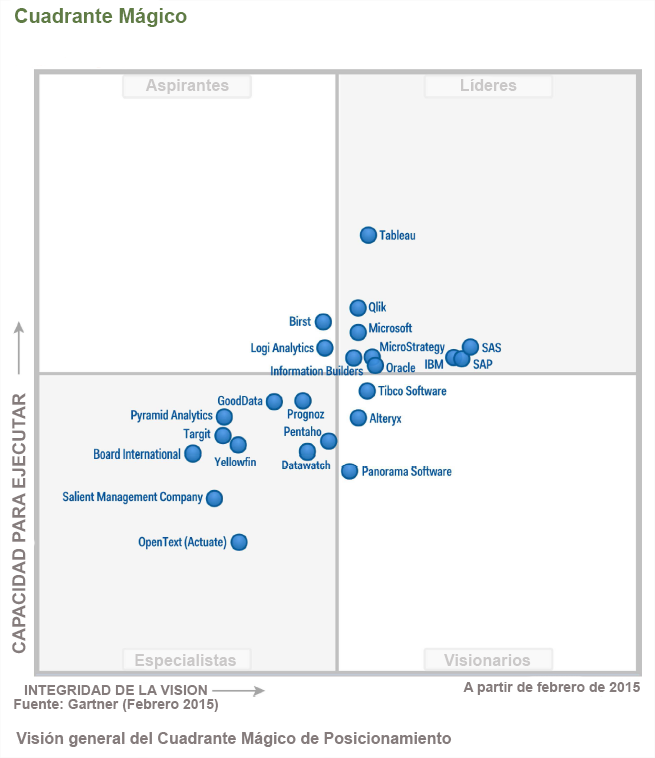
\includegraphics[width=160mm]{Magic-Quadrant.png}
	\caption{Cuadrante M�gico para BI y Plataformas Anal�ticas}
	\label{fig:magicQuadrant}
\end{figure}}

%\subsection{Tableau}
%Tableau tiene una posici�n fuerte en capacidad de ejecuci�n en el eje de l�deres del cuadrante. Esta herramienta fue la que mejor se adecu� a las necesidades del trabajo de Tesis, dado que cuenta con una versi�n p�blica para la construcci�n y publicaci�n de dashboards, adem�s de la facilidad de uso que nos proporciona. Tableau Desktop, la cual se basa en tecnolog�a drag and drop (arrastrar y soltar) permite analizar datos r�pidamente y permite ver los cambios en tiempo real sin necesidad de codificaci�n, de esta manera, posibilita a un usuario con no muchos conocimientos t�cnicos poder utilizarlo con mayor facilidad.

Los l�deres del mercado se encuentran siempre en el cuadrante superior derecho. Se puede observar una amplia diferencia entre Tableau y los dem�s l�deres. 

En las siguientes figuras se presenta el an�lisis de Gartner que eval�a las capacidades cr�ticas que debe tener una herramienta de BI y Analytics, para adecuarse a las necesidades del mercado.


\textsc{\begin{figure}[H]
	\centering
	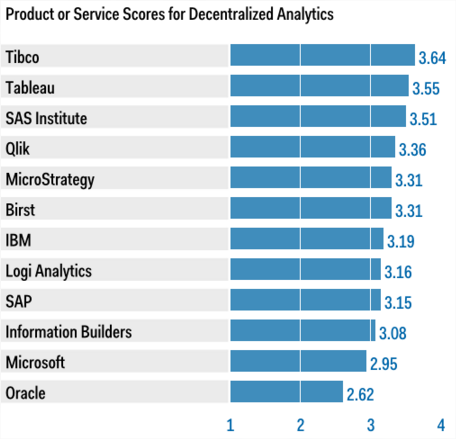
\includegraphics[width=160mm]{productOrServiceScoresForDecentralizedAnalytics.png}
	\caption{Puntuaciones de producto o servicio para an�lisis descentralizado }
	\label{fig:productOrServiceScoresForDecentralizedAnalytics}
\end{figure}}
\textsc{\begin{figure}[H]
	\centering
	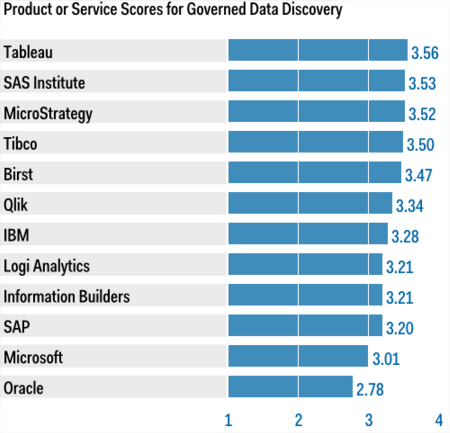
\includegraphics[width=160mm]{productOrServiceScoresForGovernedDataDiscovery.png}
	\caption{Puntuaciones de producto o servicio guiados por Data Discovery}
	\label{fig:productOrServiceScoresForGovernedDataDiscovery}
\end{figure}}


Los valores posibles van del 1 al 5, conforme la siguiente evaluaci�n: 

\begin{enumerate}
	\item Pobre o ausente: la mayor�a de los requisitos de esta capacidad no fueron alcanzadas.
	\item Justo: Algunos de los requisitos fueron alcanzados.
	\item Bueno: cumple con los requisitos.
	\item Excelente: alcanza o excede algunos requisitos.
	\item Superior: excede significativamente los requisitos.
\end{enumerate}

Tableau tiene una posici�n fuerte en capacidad de ejecuci�n (producto/servicio, su oferta, ejecuci�n de ventas, marketing, experiencia del cliente) en el eje de l�deres del cuadrante. Esta herramienta fue la que mejor se adecu� a las necesidades del trabajo de Tesis, dado que cuenta con una versi�n p�blica para la construcci�n y publicaci�n de dashboards, adem�s de la facilidad de uso que nos proporciona. Tableau Desktop, la cual se basa en tecnolog�a drag and drop (arrastrar y soltar) permite analizar datos r�pidamente y permite ver los cambios en tiempo real sin necesidad de codificaci�n, de esta manera, posibilita a un usuario con escasos conocimientos t�cnicos, poder utilizarlo de igual manera.


\textsc{\begin{figure}[H]
	\centering
	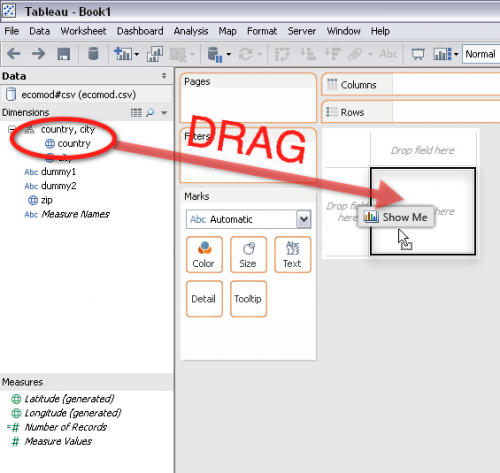
\includegraphics[width=0.7\linewidth]{figuras/tableauDragAndDrop2}
	\caption{Arrastre el campo pa�s para el campo desplegable se�alado.}
	\label{fig:tableauDragAndDrop2}
\end{figure}}



\textsc{\begin{figure}[H]
	\centering
	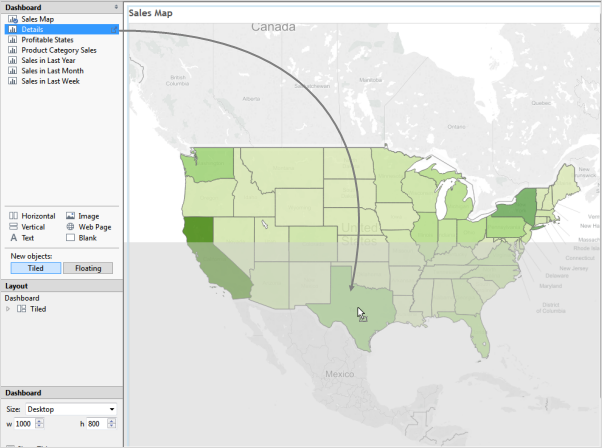
\includegraphics[width=0.7\linewidth]{figuras/tableauDragAndDrop1}
	\caption{Arrastrar hojas de trabajo al dashboard.}
	\label{fig:tableauDragAndDrop1}
\end{figure}}


De una forma �gil el usuario puede conectarse a diversas fuentes de datos y crear paneles interactivos, conectando entre s� los diferentes componentes (tipo de gr�fico) que proporciona la herramienta. La herramienta permite utilizar componentes como filtros, siendo o no de la misma fuente de datos siempre y cuando los datos coincidan en los diversos conjuntos.
Pueden ser utilizadas en la organizaciones para comprender r�pidamente diferentes aspectos del negocio. Tambi�n se puede utilizar para realizar proyecciones o tendencias,  la cual Tableau nos ofrece de manera autom�tica.
		
\section{Aplicaci�n de Data Discovery a datos de instituciones del Estado}

\begingroup
\setlength{\intextsep}{-10pt}%
\setlength{\columnsep}{8pt}%

Generalmente las organizaciones no logran comprender en su totalidad los datos que generan. La consecuencia de no comprender esos datos puede resultar en la mala toma de decisi�n, lo cual podr�a ocasionar un gran impacto negativo a la organizaci�n. La informaci�n es considerada como uno de los recursos m�s importantes en una organizaci�n, y en base a esta informaci�n, se puede obtener conocimiento que podr�a ayudar a obtener mejores resultados.

En el presente trabajo son analizados datos de la ANDE y de la DGEEC, relacionando ambos conjuntos de datos, con el objetivo de obtener informaci�n de inter�s para la organizaci�n.
\endgroup 

\subsubsection{Datos de la ANDE y de la DGEEC}

Se cuenta con datos de consumo de energ�a el�ctrica, facturaciones, grupos de consumo (residencial, industrial, exportaci�n, comercial, gubernamental y otros), por a�o (2000-2014), departamento y distrito. Estos datos fueron solicitados formalmente a la instituci�n a trav�s de la Facultad de Ciencias y tecnolog�a de la Universidad Cat�lica, la cual tuvimos una respuesta favorable para proceder.

\subsubsection{Dashboard de control / monitoramiento}
	
En esta secci�n se muestra 4 ejemplos de paneles informativos, resultantes del relacionamiento de ambos conjunto de datos.  Una de las t�cnicas utilizada para medir el crecimiento es la  ``tasa de crecimiento``, la cual se calcula el porcentaje de crecimiento que hubo por cada a�o (Ej: Si al cerrar el a�o 2014, la cantidad de clientes lleg� a 1.000.000 y en el a�o 2015 aument� 100.000, esto quiere decir que en el a�o 2015, la tasa de crecimiento de los clientes fue del 10\%, es decir, hubo un crecimiento positivo y la cantidad de clientes ha aumentado respecto al a�o anterior). Suponiendo que en el a�o 2016 la ANDE cierra con un total de 1.000.000 de clientes, su crecimiento ser�a 10\% menor al a�o anterior.
La f�rmula empleada (ver Figura ~\ref{fig:formula}), donde ``n`` es el a�o actual y ``n-1`` el a�o anterior, PIB es una variable que indica, en el caso  de nuestra comparaci�n, la cantidad de clientes que posee la ANDE .
	
\textsc{\begin{figure}[H]
	\centering
	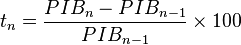
\includegraphics[width=0.7\linewidth]{figuras/formula}
	\caption{Form�la para hallar tasa de crecimiento.}
	\label{fig:formula}
\end{figure}}
	
\subsection{Dashboard - Clientes Facturados vs Crecimiento Poblacional}
Este dashboard se realiz� a fin de cruzar los datos del DGEEC y la ANDE, se utilizan datos hist�ricos de la poblaci�n y datos de clientes, consumo e importe de la ANDE.

\textsc{\begin{figure}[H]
	\centering
	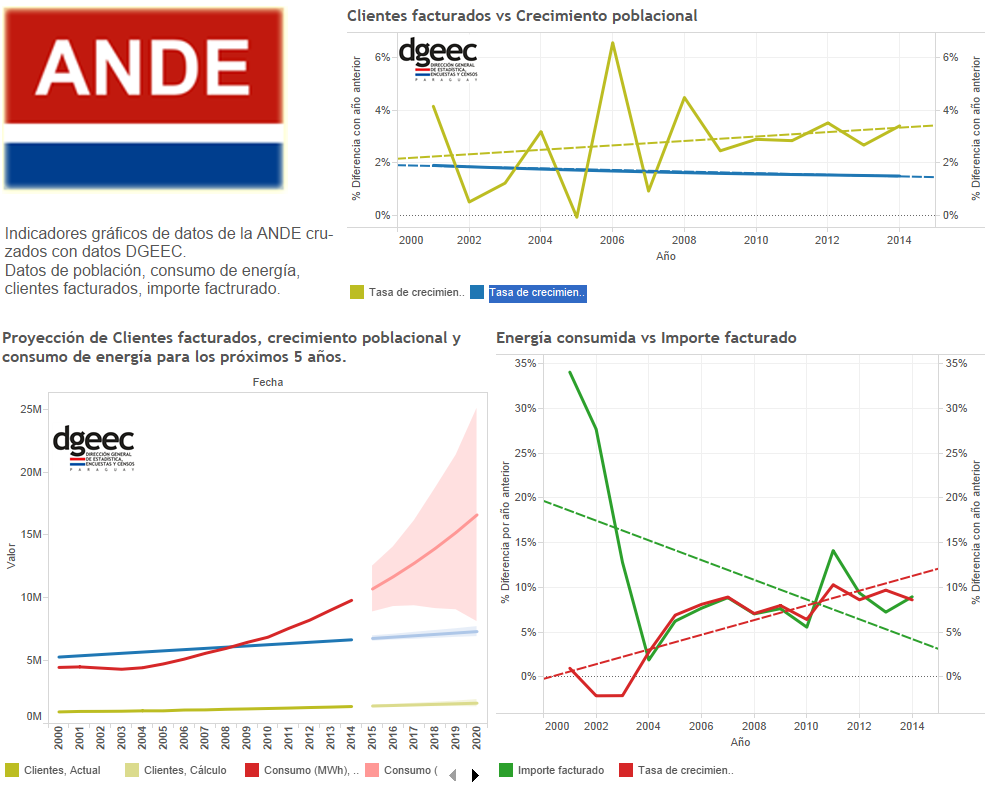
\includegraphics[width=\linewidth]{figuras/ClientesFacturadosVsCrecimientoPoblacional3}
	\caption{Clientes Facturados vs Crecimiento Poblacional}
	\label{fig:ClientesFacturadosVsCrecimientoPoblacional3}
\end{figure}}

El siguiente gr�fico representa el porcentaje del crecimiento anual de los clientes en comparaci�n con el de la poblaci�n. Podemos observar que la l�nea que pertenece a la tasa de crecimiento de la poblaci�n (azul), fue bajando al pasar los a�os. Esto no quiere decir que la poblaci�n fue disminuyendo, sino que cada a�o el porcentaje de aumento es menor.

\textsc{\begin{figure}[H]
	\centering
	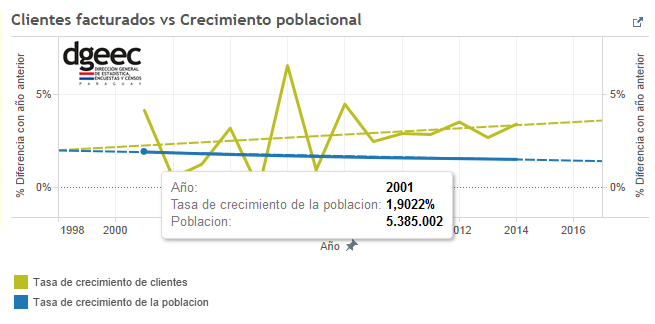
\includegraphics[width=\linewidth]{figuras/ClientesFacturadosVsCrecimientoPoblacional4}
	\caption{Clientes Facturados vs Crecimiento Poblacional}
	\label{fig:ClientesFacturadosVsCrecimientoPoblacional4}
\end{figure}}


\textsc{\begin{figure}[H]
	\centering
	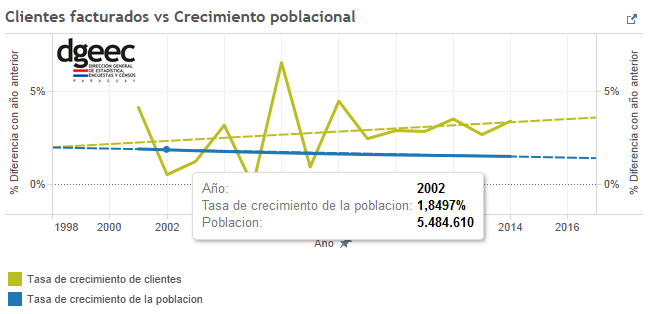
\includegraphics[width=\linewidth]{figuras/ClientesFacturadosVsCrecimientoPoblacional}
	\caption{Clientes Facturados vs Crecimiento Poblacional}
	\label{fig:ClientesFacturadosVsCrecimientoPoblacional}
\end{figure}}

La l�nea amarilla representa al porcentaje del crecimiento de los clientes de la ANDE. Como podemos ver, hay      a�os en que el aumento es muy notorio (2004,2006,2008) y hay a�os en que este es m�nimo(2002,2005,2007). Las l�neas discontinuas representan las tendencias de ambos puntos. Por ejemplo, la cantidad de clientes en el a�o 2001 fue de 959.580, la cual aument� el 4.1\% respecto al a�o anterior. 

\textsc{\begin{figure}[H]
	\centering
	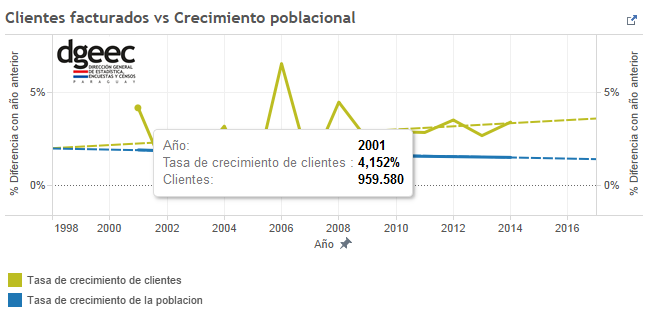
\includegraphics[width=\linewidth]{figuras/ClientesFacturadosVsCrecimientoPoblacional2}
	\caption{Clientes Facturados vs Crecimiento Poblacional}
	\label{fig:ClientesFacturadosVsCrecimientoPoblacional2}
\end{figure}}

En el a�o 2002 la cantidad de clientes ascendi� a 964.449 con un aumento de 4.869, que corresponde a un incremento     del 0.5\% respecto  al a�o 2001. Sin embargo, en el a�o 2003 el incremento fue de 1.\%, la cual representa a un aumento de m�s que el doble del a�o anterior.


\textsc{\begin{figure}[H]
	\centering
	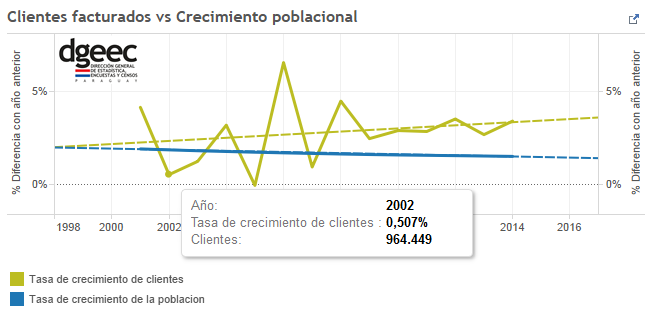
\includegraphics[width=\linewidth]{figuras/ClientesFacturadosVsCrecimientoPoblacional5}
	\caption{Clientes Facturados vs Crecimiento Poblacional}
	\label{fig:ClientesFacturadosVsCrecimientoPoblacional5}
\end{figure}}

\textsc{\begin{figure}[H]
	\centering
	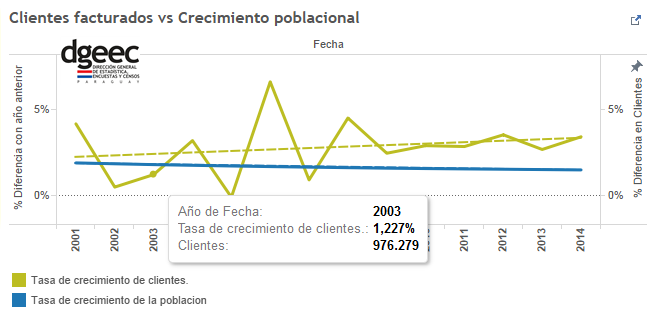
\includegraphics[width=\linewidth]{figuras/ClientesFacturadosVsCrecimientoPoblacional6}
	\caption{Clientes Facturados vs Crecimiento Poblacional}
	\label{fig:ClientesFacturadosVsCrecimientoPoblacional6}
\end{figure}}

En el siguiente gr�fico se realiza una proyecci�n o forecasting donde se muestra que probablemente, si la entidad conserva la misma cantidad de clientes o estos crecen m�nimamente, de igual manera el consumo podr�a aumentar o disminuir dr�sticamente. El aumento dr�stico del consumo, podr�a deberse al aumento de productos electr�nicos que consumen mucha m�s energ�a el�ctrica y tambi�n a que el poder adquisitivo de cada ciudadano ha aumentado. Este comportamiento se observa en la zona de c�lculo de proyecci�n (rojo, azul y amarillo suavizado).



\textsc{\begin{figure}[H]
	\centering
	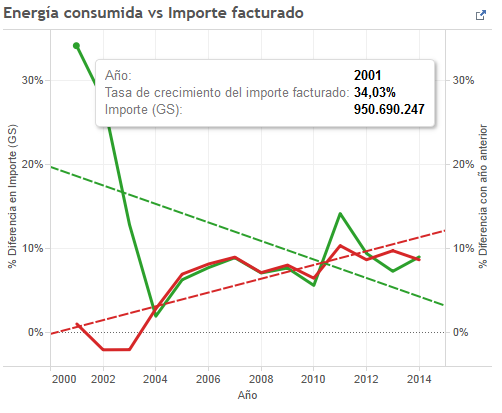
\includegraphics[width=\linewidth]{figuras/EnergiaConsumidaVsImporteFacturado}
	\caption{Energ�a Consumida vs Importe Facturado}
	\label{fig:EnergiaConsumidaVsImporteFacturado}
\end{figure}}

En el tercer y �ltimo gr�fico de este panel, se muestra la porcentaje del crecimiento anual de los importes facturados y consumo de energ�a. Se puede observar que la facturaci�n de la ANDE acompa�a al consumo de energ�a el�ctrica, exceptuando el a�o 2011, en la cual el importe aument� mas de lo que aument� el consumo de energ�a, sin embargo en el a�o 2013 el importe volvi� a aumentar menos que antes.

\textsc{\begin{figure}[H]
	\centering
	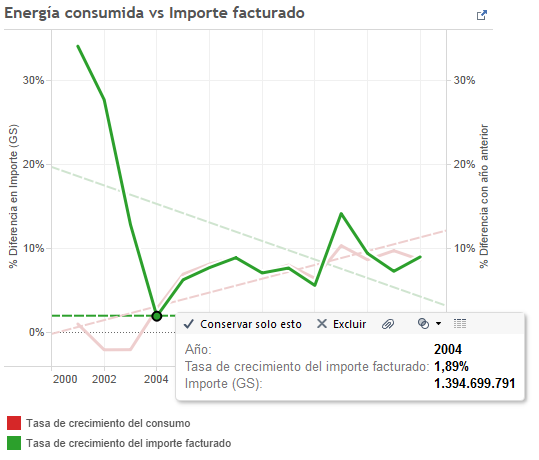
\includegraphics[width=\linewidth]{figuras/EnergiaConsumidaVsImporteFacturado2}
	\caption{Energ�a Consumida vs Importe Facturado}
	\label{fig:EnergiaConsumidaVsImporteFacturado2}
\end{figure}}


\textsc{\begin{figure}[H]
		\centering
		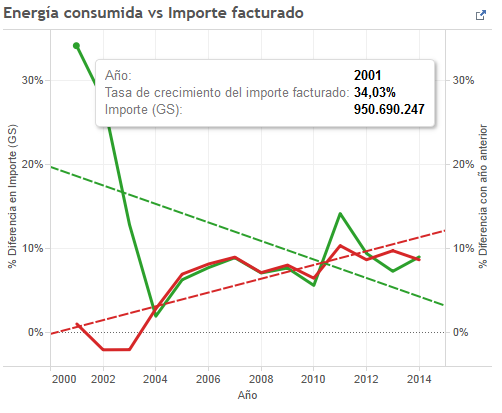
\includegraphics[width=\linewidth]{figuras/EnergiaConsumidaVsImporteFacturado3}
		\caption{Energ�a Consumida vs Importe Facturado}
		\label{fig:EnergiaConsumidaVsImporteFacturado3}
	\end{figure}}
\subsubsection{Panel estad�stico de consumo de electricidad por sector}

En la figura ~\ref{fig:EstadisticaDeConsumoDeElectricidadPorSector1990-2014} se presenta un gr�fico con el consumo de energ�a hist�rica, que abarca desde el a�o 1990 hasta 2014. Estos datos est�n clasificados por los siguientes criterios de la ANDE: Alumbrado P�blico, Comercial, Exportaci�n, Gubernamental, Industrial y Residencial. En este gr�fico se puede apreciar que el mayor consumo de energ�a se encuentra en el sector Residencial. Sin embargo, los valores de Exportaci�n de energ�a fue disminuyendo durante el tiempo. Esto tiene sentido debido a que ambos valores son inversamente proporcionales, esto es, cuando el consumo nacional se incrementa, se hace un mayor uso de energ�a en el pa�s, por lo tanto disminuye la energ�a disponible para exportaci�n.


\textsc{\begin{figure}[H]
	\centering
	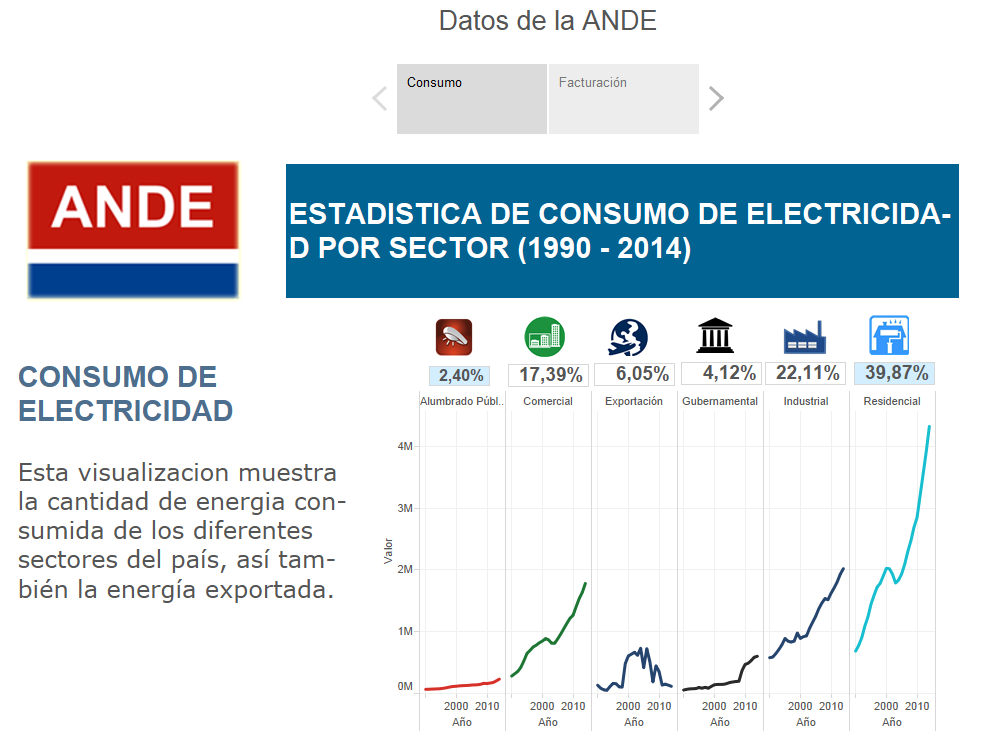
\includegraphics[width=\linewidth]{figuras/EstadisticaDeConsumoDeElectricidadPorSector1990-2014}
	\caption{Estad�stica de consumo de electricidad por sector(1990-2014)}
	\label{fig:EstadisticaDeConsumoDeElectricidadPorSector1990-2014}
\end{figure}}

La Figura ~\ref{fig:ImporteFacturadoPorAnoYSector1990-2014} presenta las informaciones de facturaci�n tambi�n clasificados por sector, con el recurso de filtros por a�o. Es importante destacar un factor resaltante: aunque energ�a exportada disminuy�, el valor facturado por energ�a vendida al exterior aument�. Es probable que esto se haya debido al aumento de la tarifa de energ�a vendida, lo cual beneficia al pa�s.


\textsc{\begin{figure}[H]
	\centering
	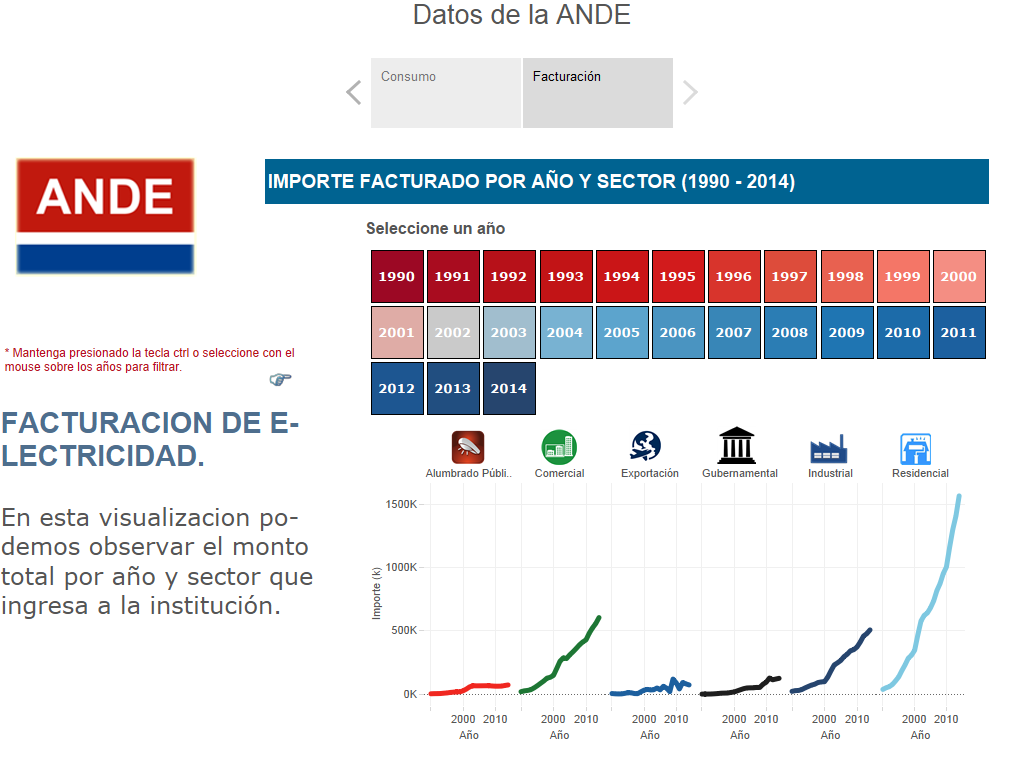
\includegraphics[width=\linewidth]{figuras/ImporteFacturadoPorAnoYSector1990-2014}
	\caption{Importe facturado por a�o y sector(1990-2014)}
	\label{fig:ImporteFacturadoPorAnoYSector1990-2014}
\end{figure}}
\subsubsection{Panel comparativo de Tasa de crecimiento y el Consumo de energ�a}

En la figura ~\ref{fig:TasaDeCrecimientoVsConsumoDeEnergia} se presenta un panel comparativo entre la tasa de crecimiento de clientes y consumo de energ�a. Tambi�n se cuenta con un mapa para filtrar por regi�n del pa�s. 

\textsc{\begin{figure}[H]
	\centering
	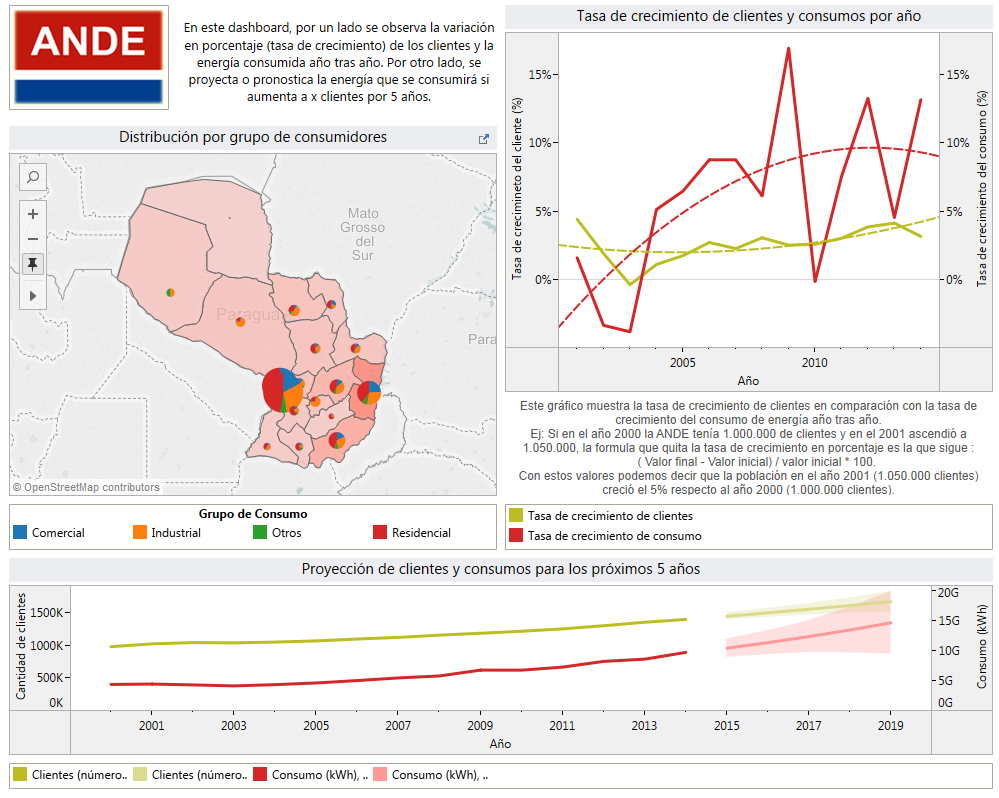
\includegraphics[width=\linewidth]{figuras/TasaDeCrecimientoVsConsumoDeEnergia}
	\caption{Tasa de crecimiento vs Consumo de energ�a}
	\label{fig:TasaDeCrecimientoVsConsumoDeEnergia}
\end{figure}}

En el gr�fico situado a la derecha del mapa (~\ref{fig:TasaDeCrecimientoVsConsumoDeEnergia2}), se tiene el consumo y crecimiento de clientes. Para un mejor analisis fue necesario suavizar los datos calculando lineas de tendencia, debido a una inestabilidad de los datos de consumo. As� se puede apreciar, que existe una tendencia de crecimiento sostenido durante el tiempo de clientes. Sin embargo, la tendencia que el consumo crezca es mayor al de clientes.

\textsc{\begin{figure}[H]
	\centering
	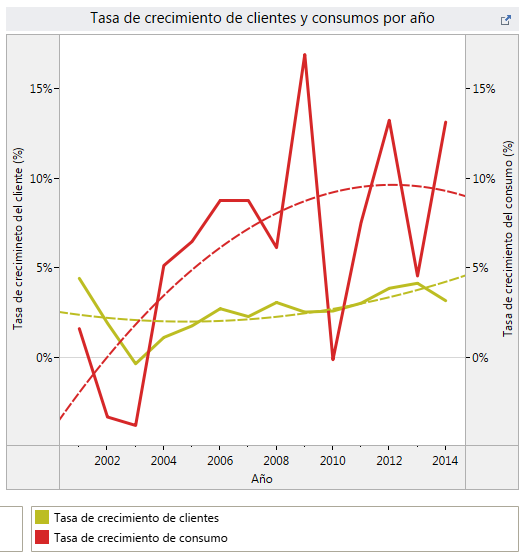
\includegraphics[width=\linewidth]{figuras/TasaDeCrecimientoVsConsumoDeEnergia2}
	\caption{Tasa de crecimiento vs Consumo de energ�a, filtrado por el departamento Alto Paran�}
	\label{fig:TasaDeCrecimientoVsConsumoDeEnergia2}
\end{figure}}

Debajo se presenta un cuadro con la l�nea de cada valor (Figura ~\ref{fig:ProyeccionDeClientesYConsumosParaLosProximos5Anos}), de crecimiento y consumo. Con el uso de un recurso disponible que cuenta la herramienta escogida Tableau, es posible realizar an�lisis predictivo  (forecasting) del crecimiento y consumo. Tableau utiliza un algoritmo llamado Suavizado Exponencial, muy conocido en el �rea de Matem�ticas Estad�sticas. En este gr�fico se puede notar que existe una mayor probabilidad que en los pr�ximos a�os aumente considerablemente el consumo, superando su media. Sin embargo, se nota que el ritmo de crecimiento de clientes es sostenible, y no tiene una alta probabilidad de sufrir un aumento abrupto.

\textsc{\begin{figure}[H]
		\centering
		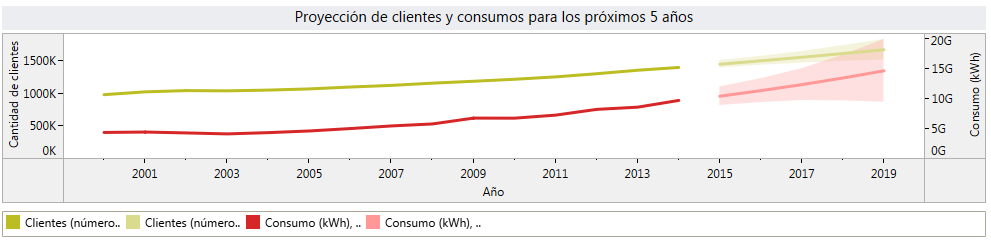
\includegraphics[width=\linewidth]{figuras/ProyeccionDeClientesYConsumosParaLosProximos5Anos}
		\caption{Proyecci�n de clientes y consumos para los pr�ximos 5 a�os}
		\label{fig:ProyeccionDeClientesYConsumosParaLosProximos5Anos}
	\end{figure}}
	
\subsubsection{Dashboard - Tasa de crecimiento poblacional vs Consumo de energ�a a�o tras a�o}

\textsc{\begin{figure}[H]
	\centering
	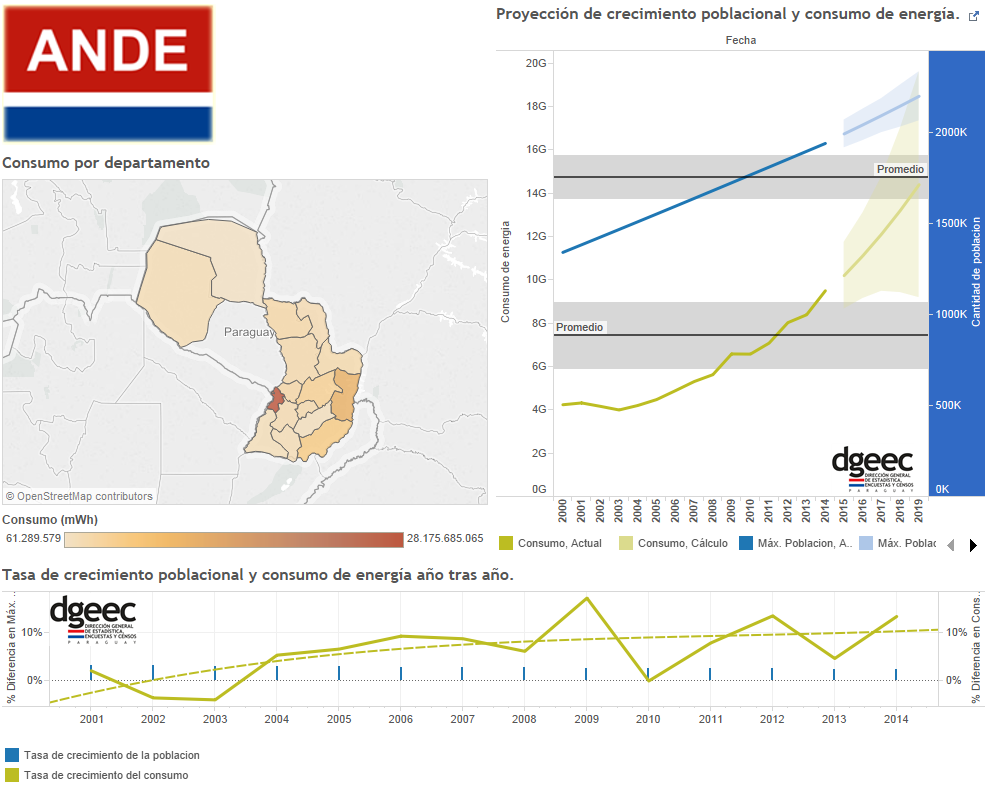
\includegraphics[width=\linewidth]{figuras/TasaDeCrecimientoPoblacionalYConsumoDeEnergiaAnoTrasAno}
	\caption{Dashboard - Tasa de crecimiento poblacional vs consumo de energ�a a�o tras a�o}
	\label{fig:TasaDeCrecimientoPoblacionalYConsumoDeEnergiaAnoTrasAno}
\end{figure}}

En el mapa, donde el color m�s oscuro representa al departamento que consume m�s energ�a el�ctrica y el color m�s claro, al que consume menos, vemos que los departamentos central, Alto Paran� son los que m�s demandan energ�a. Este tipo de gr�fico es muy �til cuando la informaci�n se quiere analizar de forma macro y georeferenciada. Al ubicar el mouse sobre cualquier departamento, se muestra un pop up indicando el valor de consumo del departamento seleccionado. Al dar clic sobre un departamento los dem�s gr�ficos tambi�n se actualizar�n en base a la selecci�n.

\textsc{\begin{figure}[H]
	\centering
	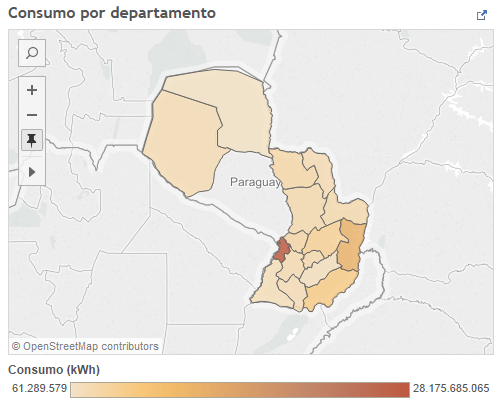
\includegraphics[width=\linewidth]{figuras/TasaDeCrecimientoPoblacionalYConsumoDeEnergiaAnoTrasAnoMapa}
	\caption{Consumo por departamento}
	\label{fig:TasaDeCrecimientoPoblacionalYConsumoDeEnergiaAnoTrasAnoMapa}
\end{figure}}

 En el segundo gr�fico, titulado ``Proyecci�n de crecimiento poblacional y consumo de energ�a``,  vemos el crecimiento de la poblaci�n (n�meros) y el crecimiento del consumo de energ�a el�ctrica expresado en GWh. Al seleccionar un departamento en el mapa, se puede analizar esta informaci�n por cada uno de ellos.


\textsc{\begin{figure}[H]
	\centering
	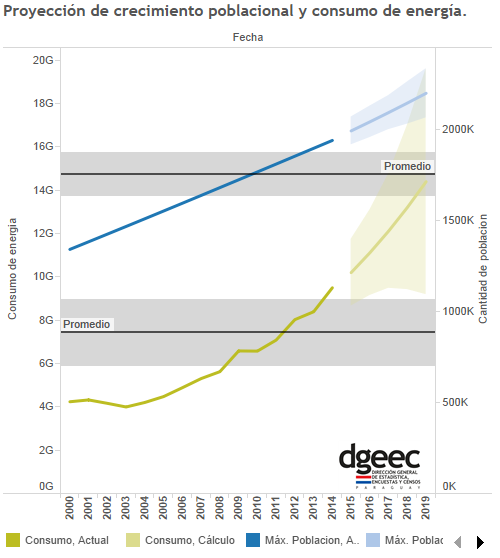
\includegraphics[width=\linewidth]{figuras/ProyeccionDeCrecimientoPoblacionalYConsumoDeEnergia}
	\caption{Proyecci�n de crecimiento poblacional y consumo ee energ�a}
	\label{fig:ProyeccionDeCrecimientoPoblacionalYConsumoDeEnergia}
\end{figure}}

En este gr�fico,  se muestra la misma informaci�n que el gr�fico anterior pero con diferente perspectiva, en este caso se calcula el porcentaje de crecimiento anual tanto de la poblaci�n, as� como del consumo.


\textsc{\begin{figure}[H]
	\centering
	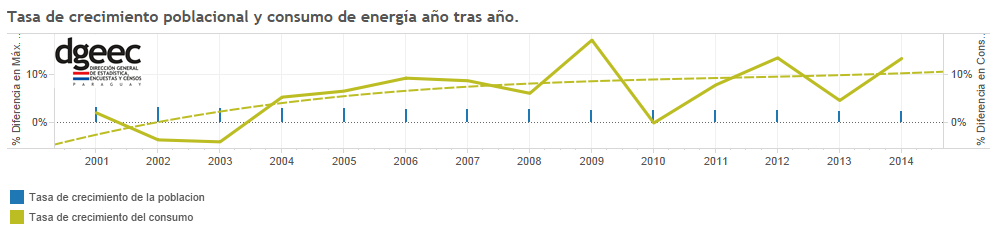
\includegraphics[width=\linewidth]{figuras/ProyeccionDeClientesYConsumosParaLosProximos5Anos2}
	\caption{Tasa de crecimiento poblacional y consumo ee energ�a a�os tras a�os}
	\label{fig:ProyeccionDeClientesYConsumosParaLosProximos5Anos2}
\end{figure}}

		\pagebreak
\chapter{CAPITULO 4}
\section{Marco Metodol�gico}
\subsection{Alcance}
Aplicaremos las t�cnicas de Data Discovery a los datos de dos instituciones del estado, espec�ficamente la \gls{sig:ANDE} y \gls{sig:DGEEC}, donde demostraremos que con datos de calidad podr�amos detectar oportunidades que nos faciliten la toma de decisiones en la instituci�n. Utilizaremos conjuntos de datos de las instituciones mencionadas m�s arriba para este fin.
\subsection{Enfoque}	
El enfoque que utilizamos es el cuantitativo, que por lo com�n, utiliza la recolecci�n y el an�lisis de datos para contestar
preguntas de investigaci�n y probar hip�tesis establecidas previamente, y conf�a en la medici�n num�rica, el conteo, y en el uso de la estad�stica para intentar establecer con exactitud  patrones en una poblaci�n. (por ejemplo un censo es un enfoque cuantitativo del estudio demogr�fico de la poblaci�n de un pa�s).
\subsection{T�cnica e Instrumentos de recolecci�n de datos}
La t�cnica aplicada en este trabajo en la recolecci�n de datos fue la investigaci�n de documentos cient�ficos procedentes de publicaciones de empresas pioneras en Data Discovery y de expertos en el �rea.

		\pagebreak
\chapter{CAPITULO 5}
\section{Conclusiones y Trabajos futuros}
Este trabajo fue dividido en las siguientes partes:


- Cap�tulo 1: en este cap�tulo fue presentada una introducci�n a los objetivos de este trabajo.

- Cap�tulo 2: Marco Te�rico: esta secci�n desarrolla el estado del arte en el �rea de BI y principalmente el de Data Discovery, t�cnica aplicada en este trabajo.

- Cap�tulo 3: En esta secci�n se presenta la evaluaci�n t�cnica realizada para la selecci�n de la herramienta Tableau. Adem�s la aplicaci�n de t�cnicas de Data Discovery a los datos de la ANDE y la DGEEC. Tambi�n se presentan los productos construidos en este trabajo, para el an�lisis de las informaciones, y las proyecciones realizadas para los pr�ximos a�os.

- Cap�tulo 4: ........

Para el desarrollo de este trabajo se obtubieron datos de la ANDE y la DGEEC. Con estos datos fue posible aplicar t�cnicas de Data Discovery realizar un analisis de las informaciones, cruzarlos, georeferenciarlos, encontrar l�neas de tendencias y pron�sticos de crecimiento a futuro tanto del consumo de energ�a, de clientes de la ANDE y de la poblaci�n del pa�s. En cada caso se presenta un an�lisis que demuestra con gr�ficos intuitivos que en ciertas ocasiones no existe una relacion proporcional entra algunas dimensiones. Sin embargo, teniendo en cuenta los resultados obtenidos se pueden observar las siguientes cuestiones:

- La tasa de crecimiento del consumo es mayor a la tasa de aumento de clientes 
- Debido a este aumento en el consumo de energ�a del pa�s, disminuy� la cantidad de energ�a exportada.
- Aunque se tuvo una disminuci�n en la energ�a exportada, se obtuvo un crecimiento en el valor facturado. Esto demuestra una mejor�a en el precio de venta de la energ�a al Brasil (Itaipu) o Argentina (Yacyreta).
- Seg�n el pron�stico de crecimiento para los pr�ximos a�os, el consumo de energ�a tendr� un crecimiento mayor al de la cantidad de clientes, y la poblaci�n del pa�s.
- La tasa de crecimiento de la poblaci�n se mantiene constante durante el tiempo, esto es, la poblaci�n crece a una tasa sostenida. Sin embargo, la tasa de aumento en el consumo de energ�a es considerablemente mayor, y demuestra un aumento abrupto para los pr�ximos a�os, independiente a la tasa de aumento de la poblaci�n y de nuevos clientes de la ANDE.


Teniendo en cuenta estas cuestiones, este trabajo puede servir de herramienta para la Planificaci�n en la Inversi�n en la capacidad de transmisi�n y distribuci�n de electricidad dentro del territorio del pa�s, para los pr�ximos a�os, adem�s de ayudar con indicadores para montar una estrategia de exportaci�n para replantear las condiciones actuales de venta de la energ�a al exterior.

		%GLOSARIO		
		\clearpage		
		\printglossary[style=mylong,title=Lista de Siglas y Acr�nimos]		
		
		\clearpage
		\renewcommand{\bibname}{Bibliograf�a}
		\bibliographystyle{apacite}
		\bibliography{bibliografia/bibFile}
	
\end{document}